%% Copernicus Publications Manuscript Preparation Template for LaTeX Submissions
%% ---------------------------------
%% This template should be used for copernicus.cls
%% The class file and some style files are bundled in the Copernicus Latex Package, which can be downloaded from the different journal webpages.
%% For further assistance please contact Copernicus Publications at: production@copernicus.org
%% https://publications.copernicus.org/for_authors/manuscript_preparation.html


%% Please use the following documentclass and journal abbreviations for preprints and final revised papers.

%% 2-column papers and preprints
\documentclass[bg, manuscript]{copernicus}



%% Journal abbreviations (please use the same for preprints and final revised papers)


% Advances in Geosciences (adgeo)
% Advances in Radio Science (ars)
% Advances in Science and Research (asr)
% Advances in Statistical Climatology, Meteorology and Oceanography (ascmo)
% Annales Geophysicae (angeo)
% Archives Animal Breeding (aab)
% Atmospheric Chemistry and Physics (acp)
% Atmospheric Measurement Techniques (amt)
% Biogeosciences (bg)
% Climate of the Past (cp)
% DEUQUA Special Publications (deuquasp)
% Drinking Water Engineering and Science (dwes)
% Earth Surface Dynamics (esurf)
% Earth System Dynamics (esd)
% Earth System Science Data (essd)
% E&G Quaternary Science Journal (egqsj)
% EGUsphere (egusphere) | This is only for EGUsphere preprints submitted without relation to an EGU journal.
% European Journal of Mineralogy (ejm)
% Fossil Record (fr)
% Geochronology (gchron)
% Geographica Helvetica (gh)
% Geoscience Communication (gc)
% Geoscientific Instrumentation, Methods and Data Systems (gi)
% Geoscientific Model Development (gmd)
% History of Geo- and Space Sciences (hgss)
% Hydrology and Earth System Sciences (hess)
% Journal of Bone and Joint Infection (jbji)
% Journal of Micropalaeontology (jm)
% Journal of Sensors and Sensor Systems (jsss)
% Magnetic Resonance (mr)
% Mechanical Sciences (ms)
% Natural Hazards and Earth System Sciences (nhess)
% Nonlinear Processes in Geophysics (npg)
% Ocean Science (os)
% Polarforschung - Journal of the German Society for Polar Research (polf)
% Primate Biology (pb)
% Proceedings of the International Association of Hydrological Sciences (piahs)
% Safety of Nuclear Waste Disposal (sand)
% Scientific Drilling (sd)
% SOIL (soil)
% Solid Earth (se)
% The Cryosphere (tc)
% Weather and Climate Dynamics (wcd)
% Web Ecology (we)
% Wind Energy Science (wes)


%% \usepackage commands included in the copernicus.cls:
%\usepackage[german, english]{babel}
%\usepackage{tabularx}
%\usepackage{cancel}
%\usepackage{multirow}
%\usepackage{supertabular}
%\usepackage{algorithmic}
%\usepackage{algorithm}
%\usepackage{amsthm}
%\usepackage{float}
%\usepackage{subfig}
%\usepackage{rotating}


\begin{document}

\title{A process-based model for quantifying the effects of canal blocking on water table and CO2 emissions in  tropical peatlands}


% \Author[affil]{given_name}{surname}

\Author[1,2]{Iñaki}{Urzainki}
\Author[3]{Marjo}{Palviainen}
\Author[4]{Hannu}{Hökkä}
\Author[5]{Sebastian}{Persch}
\Author[5]{Jeffrey}{Chatellier}
\Author[5]{Ophelia}{Wang}
\Author[5]{Prasetya}{Mahardhitama}
\Author[5]{Rizaldy}{Yudhista}
\Author[2,3]{Annamari (Ari)}{Laurén}


\affil[1]{Natural Resources Institute Finland (Luke), Latokartanonkaari 9, FI-00790 Helsinki, Finland}
\affil[2]{School of Forest Sciences, Faculty of Science and Forestry, University of Eastern Finland, Joensuu Campus, P.O. Box 111, (Yliopistokatu 7), FI-80101 Joensuu, Finland}
\affil[3]{University of Helsinki, Department of Forest Ecology, P.O. Box 27, FI-00014 Helsinki, Finland}
\affil[4]{Natural Resources Institute Finland, Oulu, Paavo Havaksen tie 3, FI-90570 Oulu, Finland}
\affil[5]{Forest Carbon PTE LTD, Singapore}

\correspondence{Iñaki Urzainki (inaki.urzainqui@luke.fi)}

\runningtitle{TEXT}

\runningauthor{TEXT}





\received{}
\pubdiscuss{} %% only important for two-stage journals
\revised{}
\accepted{}
\published{}

%% These dates will be inserted by Copernicus Publications during the typesetting process.


\firstpage{1}

\maketitle



\begin{abstract}
Drainage in tropical peatlands increases CO\textsubscript{2} emissions, the rate of subsidence, and the risk of forest fires.
To a certain extent, these effects can be mitigated by raising the water table depth (WTD) using canal or ditch blocks.
The performance of canal blocks in raising WTD is, however, poorly understood, because the WTD monitoring data is limited and spatially concentrated around canals and canal blocks.
This raises the following question: how effective are canal blocks in raising the WTD over large areas?
In this work we composed a process-based hydrological model to assess the peatland restoration performance of 168 canal blocks in a 22000 \unit{ha} peatland area in Sumatra, Indonesia.
We simulated daily WTD over one year using an existing canal block setup and compared it to  the situation without  blocks.
The study was performed across two contrasting weather scenarios representing dry (1997) and wet (2013) years.
Our simulations revealed that while canal blocks had a net positive impact on WTD rise, they lowered WTD in some areas, and the extent of their effect over one year was limited to a distance of about 600 \unit{m} around the canals.
We also show that canal blocks are most effective in peatlands with high hydraulic conductivity.
Averaging over all modelled scenarios,  blocks raised the annual mean WTD by only 1.5 \unit{cm}.
This value was similar in the dry year (1.44 \unit{cm}) and in the wet year (1.57 \unit{cm}), and there was a 2.13 fold difference between the scenarios with the maximum and minimum hydraulic conductivity (2.05 \unit{cm} versus 0.96 \unit{cm}).
Using a linear relationship between WTD and CO\textsubscript{2} emissions, we estimated that, averaging over peat hydraulic properties, canal blocks prevented the emission of 1.07 \unit{Mg ha^{-1}} CO\textsubscript{2} in the dry year and 1.17 \unit{Mg ha^{-1}} CO\textsubscript{2} in the wet year.
We believe that the  modelling tools developed in this work could be adopted by local stakeholders aiming at a more effective and evidence-based approach to canal block based peatland restoration.
\end{abstract}


\introduction  %% \introduction[modified heading if necessary]

Tropical peatlands contain approximately one sixth of the global soil carbon pool \citep{pageGlobalRegionalImportance2011, pageAnthropogenicImpactsLowland2022, xuPEATMAPRefiningEstimates2018}.
In the recent decades, extensive tropical peatland areas have been converted to agricultural and plantation forest production \citep{miettinenLandCoverDistribution2016, wijedasaCarbonEmissionsSouthEast2018}.
This land use change has often been driven by drainage, which involves excavating canals or ditches in the peat.
Canals help to remove water from the naturally waterlogged peat, enhancing site productivity, and  opening pathways for wood and crop transportation \citep{dohongReviewDriversTropical2017}.
However, the same mechanisms that make the drainage-based bioproduction economically valuable have severe environmental consequences.
Drainage increases CO\textsubscript{2} emissions \citep{novitaGeographicSettingGroundwater2021, jauhiainenCarbonDioxideEmissions2012, ishikuraSoilCarbonDioxide2018, carlsonModelingRelationshipsWater2015}, the rate of peat subsidence \citep{evansLongtermTrajectoryTemporal2022, evansRatesSpatialVariability2019, hooijerSubsidenceCarbonLoss2012, sinclairEffectsDistanceCanal2020, hoytWidespreadSubsidenceCarbon2020}, fire risk \citep{miettinenFireDistributionPeninsular2017, kielyAssessingCostsIndonesian2021}, nutrient release  \citep{laurenNutrientBalanceTool2021} and nutrient export to water courses, and decreases the peat substrate quality \citep{kononenDeforestedDrainedTropical2018}.

Drainage lowers the peatland water table depth (WTD, meters, negative downward), which activates mechanisms that are behind the environmental drawbacks.
The lower WTD increases the oxygen supply that soil microorganisms need for aerobic decomposition of organic matter \citep{pageAnthropogenicImpactsLowland2022}. 
It is as a result of the decomposition process that CO\textsubscript{2} is emitted, peat subsides, and nutrients are released.
Therefore, raising the WTD has been the focus of many restoration practices.
Canal blocks or dams raise the canal water level (CWL), increase the residence time of water in the peatland, and raise the WTD in the peat \citep{dohongReviewTechniquesEffective2018}.

Despite the widespread use of canal blocks for peatland restoration, there exists little evidence for their effectiveness, especially   in large areas.
Most existing studies monitor WTD before and after block installation using dipwells.
Due to practical restrictions, dipwells are usually installed close to the canals, which is the area where WTD rise due to canal blocks is expected to be largest \citep{sutiknoWaterManagementHydrological2020, kasihRewettingDegradedTropical2016, ritzemaCanalBlockingStrategies2014}.
As a result, a naive extrapolation of the observed  block-induced WTD response to larger scales will likely result in overestimating their effectiveness.
Moreover, since WTD depends on variable meteorological factors and complex hydrological processes, the difference between WTD before and after building the blocks cannot be directly attributed to their presence.
In their review about tropical peatland restoration practices, \cite{dohongReviewTechniquesEffective2018} concluded that while nearly all canal blocking studies have reported that the WTD rose after the dams were placed, "our current knowledge and skills are arguably inadequate for the large and landscape scale peatland restoration in Indonesia".

Process based models offer a different, complementary approach to analyze WTD response to blocks.
If implemented correctly, the models can account for the complex, interconnected factors affecting the canal block WTD response in large areas, which include peat topography, canal topology and block location, peat hydraulic properties, and  rainfall patterns.
They also enable a direct comparison of WTD between different blocking setups.
Process based models have been applied to simulate WTD in tropical peatlands in multiple studies \citep{wostenTropicalPeatlandWater2006, cobbHowTemporalPatterns2017, bairdHighPermeabilityExplains2017, urzainkiCanalBlockingOptimization2020}.
Only few of those have dealt with the question of block performance  \citep{jaenickePlanningHydrologicalRestoration2010, ishiiGroundwaterPeatland2016, putraModellingPerformanceBunds2022}.
The studies by \cite{ishiiGroundwaterPeatland2016} and \cite{jaenickePlanningHydrologicalRestoration2010} did not consider different peat hydraulic properties or weather scenarios, therefore limiting the generalizability of their results.
\cite{putraModellingPerformanceBunds2022}, on the other hand, presented a good experimental setup to analyze block and bund efficiency, but their simulations were confined to an area of $20$ \unit{ha}.
Notwithstanding the usefulness of their approach to plan small-scale mitigation strategies and to understand restored peatland WTD dynamics, such small scales are insufficient for assessing the rewetting abilities of blocks over regional scales.

The aim of the present study is to assess the effectiveness of canal blocking restoration practices for a large tropical peatland area ($22000$ \unit{ha}) in Sumatra, Indonesia, using a process-based hydrological model.
We seek to understand the scale of the block impact under different weather conditions and  peat hydraulic properties.
To meet that challenge, we constructed a new hydrological model that combines the diffusive wave approximation of the open channel flow equations with the groundwater flow equation that solves the WTD throughout the peatland area.
The model for the CWL is sensitive to the presence of canal blocks, and the spatially-explicit WTD was used to compare the blocked and non-blocked scenarios.
The results were further evaluated to assess the impact of canal blocking on CO\textsubscript{2} emissions from the tropical peat area.


\section{Materials and Methods}
\subsection{Study area}
The $22000$ \unit{ha} study area is part of an ecosystem restoration concession, the Sumatra Merang Peatland Project (SMPP), which is located in within the largest peat swamp dome in South Sumatra---the $140000$ \unit{ha} Merang-Kepayang peat dome.
The area is an ecologically significant wetland close to Berbak Sembilang National Park, and as many other swamp forests in Southeast Asia, it has been degraded by logging of the primary forest and by the construction of drainage canals.
After more than a decade of widespread illegal logging, the SMPP rehabilitation project  began in 2017 with an initial installation of 87 temporary box dams, followed by 203 permanent peat compaction dams that were constructed between 2019 and 2021.
The SMPP area remains uninhabited, and pioneering native forest species are the main vegetation cover, with only 200 ha of original peat swamp forest habitat remaining.

Our study site, a large subset of the SMPP area, contains  $219$ \unit{km} of canals and 168 dams (Figure \ref{fig:study_area}).
The locations of the peat compaction dams  were based on elevation difference by distance \citep{jaenickePlanningHydrologicalRestoration2010}.
The peat depth averages at about $5$ \unit{m}.
There are five patrol posts inside our area, each consisting of a weather station and six daily-measured dipwells along a $200$ \unit{m} transect perpendicular to the nearest canal. 
There are 111 additional dipwells measured manually at an approximately monthly frequency.
Weather and WTD data was collected for 365 days, starting from January 22nd, 2020.

\begin{figure}[H]
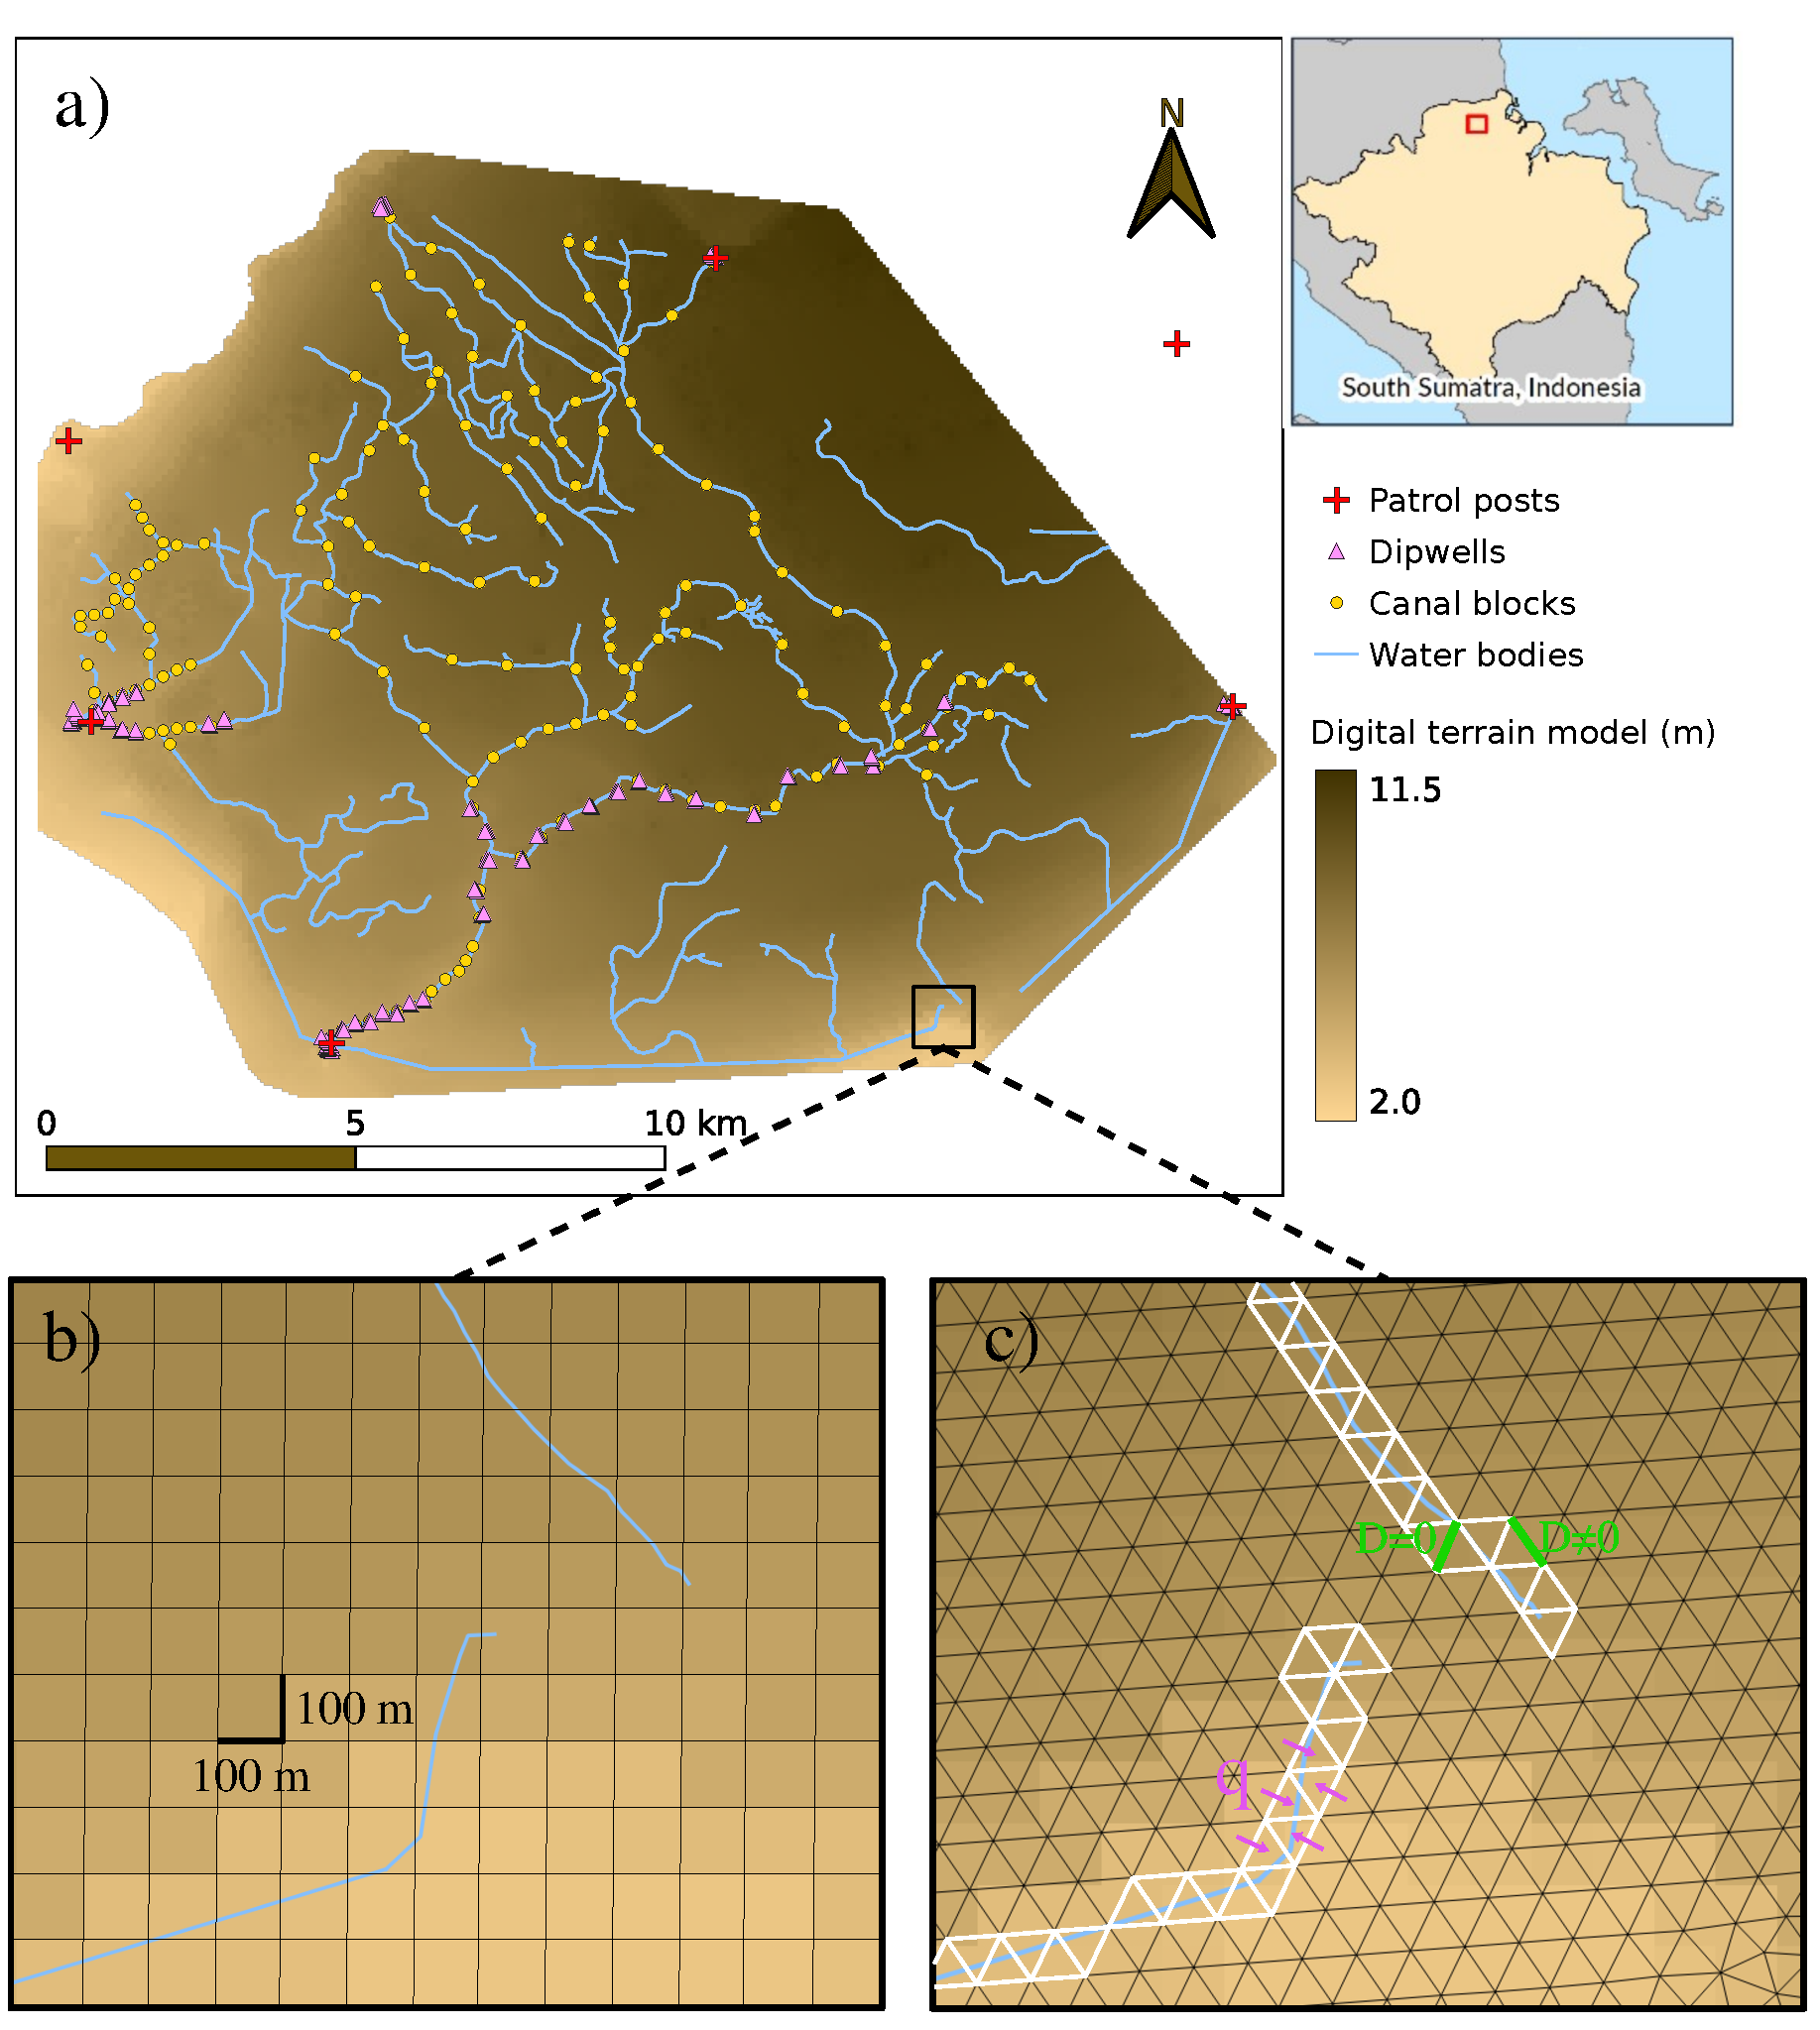
\includegraphics[width=12 cm]{figs/area+zoominDTM.pdf}
\caption{Study area and peat hydrological module (PHM) mesh. \textbf{(a)} Digital terrain model (brown gradient), water bodies (blue lines), dipwells (pink triangles), canal blocks (yellow dots) and patrol posts (red crosses). Each patrol posts consist of a weather station and six daily measured  dipwells along a 200 \unit{m} transect. The rest of the dipwells were measured manually with monthly frequency. Native forest species are the main vegetation cover. The area extends from ($2^\circ 5' 29''$ S $104^\circ 3' 14''$ E) to ($1^\circ 57' 11''$ S $104^\circ 14' 1''$ E). \textbf{(b)} and \textbf{(c)} Zoomed in region near two canals in the southern part of the study area. \textbf{(b)} Original 100 \unit{m} $\times$ 100 \unit{m} resolution of the digital terrain model, which was later interpolated to 50 \unit{m} $\times$ 50 \unit{m}. \textbf{(c)} Triangular mesh for the peat hydrological module (PHM). The white segments show the mesh cell faces corresponding to the canals, which were treated differently. This difference is emphasized with the green and pink schematic annotations. Two cell faces are shown in green: one is the face between two canal mesh cells, and consequently has no hydraulic transmissivity, $T=0$; the other is the face between a canal and a peat mesh cell and therefore $T\neq0$ in general. In pink we indicate the lateral inflow per unit length, $q$, between the peat and canal mesh cells.}
\label{fig:study_area}
\end{figure}   

    
\subsection{Modelling}
We constructed a hydrological model that produces daily WTD maps.
The model consists of a canal network module (CNM) and a peat hydrological module (PHM).
At each timestep, these modules work in an alternate fashion to update the next day’s canal water level (CWL, meters, negative downwards) and WTD across the study area.
First, the CNM computes and updates the CWL using the amount of water expected to have flowed in the peatland-canal interface, which was computed by the PHM in the previous timestep.
Then, the PHM computes and updates the WTD using the newly computed CWL.
The PHM allows for bidirectional water flow between the canals and the peatland, but it only updates the state of the WTD, not the CWL.

The CWL and the WTD are essentially the same quantity: water height above a common reference datum; therefore, they are described in this text with the same symbol, $h$.
The context is hopefully clear enough for the reader to discriminate between the two.
In the following, each module is described in more detail.

\subsubsection{Canal network module (CNM)}
The CNM solves $h$ in the canal network using a diffusive wave approximation of the open channel flow equations \citep{szymkiewiczNumericalModelingOpen2010}.
This approximation requires less computational resources than a solution of the full equations, making it particularly suitable for catchment-scale peatland areas with complex canal structures.
Additionally, it is able to describe the propagation of the water flow both in the upstream and downstream directions and thus it can represent the  upstream influence of dams, a key feature for our intended application.
The diffusive wave approximation is derived from the open channel flow equations by neglecting the two inertial terms in the momentum equation, which results in a gradient of $h$ that depends only on the friction slope \citep{novakHydraulicModellingIntroduction2010}.
Here we use a formulation of the open channel flow equations given by the water surface elevation from the reference datum, $h$ [\unit{m}], and the discharge, $Q$ [\unit{m^3s^{-1}}], with the friction slope described by Manning's equation \citep{cungePracticalAspectsComputational1980},

% Full SVE
%\begin{equation} \label{eq:SVE}
%\left\{ \begin{aligned} 
%    \frac{\partial h}{\partial t} & = -\frac{1}{B}\frac{\partial Q}{\partial x} + q \\
%    \frac{\partial Q}{\partial t}  & = -\frac{\partial}{\partial x} \left(\frac{Q^2}{A}\right) -  gA\frac{\partial h}{\partial x} - g\frac{n^2 Q |Q|}{A R^{4/3}}
%\end{aligned} \right.
%\end{equation}


\begin{align}
    \frac{\partial h}{\partial t} & = -\frac{1}{B}\frac{\partial Q}{\partial x} + \frac{q}{B} \label{eq:diff-wave-mass}\\
    \frac{\partial h}{\partial x}  & = - \frac{n^2 Q |Q|}{A^2 R^{4/3}}. \label{eq:diff-wave-momentum}
\end{align}

Here $B$ is the channel width [\unit{m}], $q$ is the lateral inflow per unit length [\unit{m^3m^{-1}s^{-1}}], $A$ is the cross-sectional flow area [\unit{m^2}], $n$ is the Manning friction coefficient [\unit{m^{-1/3}s}] and $R$ is the hydraulic radius [\unit{m}].
Our model used a simple rectangular channel of height $z$, i.e., $A = B(h-p+z)$, where $p$ [\unit{m}] is the local peat surface elevation above the reference datum.
A graphical representation of the variables is shown in Figure \ref{fig:schema_SVE}, and Table \ref{tab:rest_of_params} contains the parameter values.
The  parameters specifying canal geometry --width, depth and cross-section shape-- were determined by local expert observations.

\begin{figure}[H]
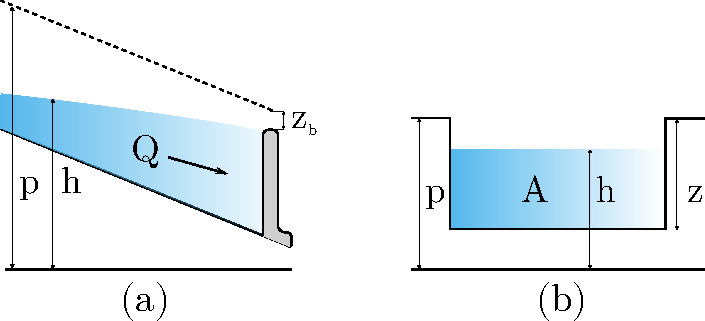
\includegraphics[width=8.3 cm]{figs/canal_alboko_goitiko_bistak.pdf}
\caption{Schematic representation of the relevant variables in the open channel flow equations. \textbf{(a)} Side view and \textbf{(b)} channel cross-section. The grey structure represents a dam.}
\label{fig:schema_SVE}
\end{figure}  


\begin{table}[t] 
\caption{Fixed parameter values across all modelled scenarios.}
\label{tab:rest_of_params} 
\begin{tabular} {c c c c l}
\tophline
\textbf{Parameter} & \textbf{Value} & \textbf{Unit} &  \textbf{Equation} & \textbf{Description} \\
\middlehline
$B$ & 1.5 & \unit{m} & \eqref{eq:diff-wave-mass} & canal width \\
$z$ & 1.5 & \unit{m} & \eqref{eq:n(h)} & canal height. Distance to canal bed measured from the local peat surface \\
$z_b$ & 0 & \unit{m} & \eqref{eq:Qblock} & Distance to the block head, measured from the local peat surface \\
$n_t$ & 100 & \unit{m^{-1/3}s} & \eqref{eq:n(h)} &  Maximum value of $n$.\\
$n_1$ & 5 & - & \eqref{eq:n(h)} & Parameter of the Manning friction coefficient\\
$n_2$ & 1 & - & \eqref{eq:n(h)} &  Parameter of the Manning friction coefficient \\
$K_b$ & 2000 & \unit{m^{3/2}s^{-1}} & \eqref{eq:Qblock} & Block discharge coefficient \\
$s_1$ & 0.6 & - & \eqref{eq:S_zeta} & Parameter of the specific yield function\\
$s_2$ & 0.5 & - & \eqref{eq:S_zeta} & Parameter of the specific yield function\\
\bottomhline
\end{tabular}
%\belowtable{} % Table Footnotes
\end{table}


The mass conservation equation, Eq.\eqref{eq:diff-wave-mass}, may be combined with the momentum equation, Eq.\eqref{eq:diff-wave-momentum}, to eliminate one of the dependent variables, $h$ or $Q$.
Usually, $h$ is eliminated to get an advection-diffusion partial differential equation (PDE) for $Q$ \citep{novakHydraulicModellingIntroduction2010, szymkiewiczNumericalModelingOpen2010}.
However, here we are interested in the water level in the canal network, and thus instead eliminate $Q$ to get a PDE for $h$.
This transformation and the resulting conservative numerical schemes are expressed in detail in Appendix \ref{ap-difwave}.

We constructed the Manning friction coefficient $n$ according to these assumptions:
\begin{itemize}
    \item The friction increases as the CWL approaches the canal bed. This is due to the resistance to water flow introduced by vegetation growing in the canals and the canal bed surface roughness.
    \item When the CWL is below the canal bed, water may still flow through the underlying peat. The friction coefficient in this zone must be several orders of magnitude higher because it is effectively describing water flow in a porous medium.
    \item The friction increases with decreasing CWL in a nonlinear fashion.
\end{itemize}
Therefore, the Manning friction coefficient was described as follows:

\begin{equation} \label{eq:n(h)}
n (h) =
	\begin{cases}
		n_t e^{- n_1 (h - p + z)^{n_2}}& h > p - z \\
		  n_t & h \leq p - z
	\end{cases}.
\end{equation}

Here $n_t$ is a threshold value of $n$ [\unit{m^{-1/3} s}], and $n_1$ and $n_2$ are parameters.
When the CWL drops below the canal bed elevation $h_b$, the Manning friction coefficient is equal to its maximum, $n_t$.
For heads above the canal bed, $n$ decreases exponentially with a shape dictated by $n_1$ and $n_2$.
In the absence of better information sources the values for these parameters were chosen so that the value of $n$ when the canal is full of water was $n = 0.055$ \unit{m^{-1/3} s}, which is in the range described in \citet{szymkiewiczNumericalModelingOpen2010}, and the value for flows below the canal bed was $n = 100$ \unit{m^{-1/3} s} (see Table \ref{tab:rest_of_params}).


The water discharge through a canal block, $Q_b$ [\unit{m^3s^{-1}}],  was modelled using the following relationship \citep{szymkiewiczNumericalModelingOpen2010},
\begin{equation} \label{eq:Qblock}
Q_b = K_b \max\left(0, h - p + z_b\right)^{1.5},
\end{equation}
where $K_b$ [\unit{m^{3/2}s^{-1}}] is a coefficient regulating the rate of water flow through the block, and $p - z_b$ [\unit{m}] is the elevation of the block head above the reference datum (Figure \ref{fig:schema_SVE}.
With this choice, the dam completely blocks water when the CWL is below the block head level.
The block discharge coefficient, $K_b$, was determined by adjusting the parameter until the flow rate was acceptable.

The challenge of solving the open channel flow equations in a large network of interconnected canals was met with a novel discretization of the equations.
As usual, each canal reach was discretized as a one dimensional grid with a fixed spacing between nodes of $\Delta x = 50 \unit{m}$.
The novelty introduced by our method concerns the canal junctions.
We exploited the basic properties of conservation equations that fully specify the governing equations at every node in the computational domain.
This is different from the usual practice, in which external mass and energy conservation equations need to be added manually to the system of equations in order to describe water flow at canal junctions \citep{cungePracticalAspectsComputational1980}.
As a result, the computational domain in our method is, by design, analogous to the canal network topology, which simplifies the implementation.
Further details on the discretization method are given in Appendix \ref{ap-difwave}.

In our implementation of the model, disconnected components of the canal network were solved independently, in parallel processes.
The accelerated Newton-Raphson method introduced by \cite{liuApplyingMicroprocessorAnalysis2014} was used to solve the resulting nonlinear system of equations.
No-flow Neumann boundary conditions were set at all boundary nodes.

\subsubsection{Peat hydrological module (PHM)}
This module uses the output from the CNM to compute the daily WTD in the peat.
The approach is  similar  to the peat hydrological module presented previously in \cite{urzainkiCanalBlockingOptimization2020} and many others before that (see, e.g., \cite{cobbHowTemporalPatterns2017, morrisDigiBogPeatlandDevelopment2012, putraModellingPerformanceBunds2022}).
We solve the two dimensional groundwater flow equation, which is suitable for domains much wider than they are thick \citep{connortonDoesRegionalGroundwaterflow1985, bearModelingGroundwaterFlow2010},

\begin{equation} \label{eq:boussinesq}
S_y(h)\frac{\partial h}{\partial t} = \nabla\left(T(h) \nabla h \right) + P - ET,
\end{equation}
where $P - ET$ [\unit{m d^{-1}}], the difference between precipitation and evapotranspiration, is the net water input to the system, $S_y$ is the specific yield, and $T$ is the peat hydraulic transmissivity [\unit{m^2d^{-1}}].

Equation \eqref{eq:boussinesq} describes water flow through a porous medium.
When water ponds above the peat surface, the medium in which water moves is no longer porous, and the physical description of the dynamics of water changes.
Our model explicitly separates the two domains (below and above ground) by using a piecewise-defined peat hydraulic transmissivity.

Both the specific yield and the transmissivity are known to vary with WTD.
This is especially true of the transmissivity, which may vary in several orders of magnitude in just a few centimetres \citep{cobbHowTemporalPatterns2017}.
Following the results of \cite{cobbScalarSimulationParameterization2019}, our model describes the nonlinear variation of $S_y$ and  $T$ in the vertical profile with exponential functions.
The specific yield was parameterized as
\begin{equation} \label{eq:S_zeta}
S_y (\zeta) = s_1 e^{s_2\zeta},
\end{equation}
where $s_1$ and $s_2$ are parameters (see Table \ref{tab:peat_property_params}), and $\zeta$ is the WTD as measured from the local peat surface [\unit{m}, negative downwards]
% When the WTD is above ground, the theoretical value of the specific yield is $S_y=1$, because a unit increase in water volume per unit area increases the WTD by the same amount.
\begin{equation} \label{eq:def_zeta}
\zeta = h - p.
\end{equation}

The transmissivity was parameterized as:
\begin{equation} \label{eq:T_zeta}
T (\zeta, d) =
	\begin{cases}
         t_1 \left( 1 + t_2\zeta - e^{-t_2 d} \right) & \zeta > 0 \\
		 t_1(e^{t_2\zeta} - e^{-t_2 d}) & \zeta \leq 0
	\end{cases}
 ,
\end{equation}
where $d$ is the local peat thickness [\unit{m}] and $t_1$ and $t_2$ are parameters (see Table \ref{tab:peat_property_params}).

Below ground, the transmissivity increases exponentially with WTD from a value of $T(\zeta = -d)=0$ when the WTD is at the bottom of the peat column. 
Above ground, on the contrary, we opted for a constant conductivity, the derivative of transmissivity ($K = \frac{\partial T}{\partial \zeta}$), which results in a linear $T(\zeta)$.
It can be checked that $T(\zeta)$ is continuous and differentiable at the domain threshold $\zeta = 0$, which helps avoid potential numerical problems.

Equation \eqref{eq:boussinesq} was solved using an explicit finite volume solver in an unstructured mesh generated from the study area maps (see Figure \ref{fig:study_area} \textbf{(c)}).
Convergence and stability of the numerical method where confirmed by solving the equation with a 42 times smaller timestep for one day (usually, $\Delta t= 1/24$ \unit{d}; $\Delta t = 1/1000$ \unit{d} was used for the tests).
Our code relied on open source software \citep{guyerFiPyPartialDifferential2009, geuzaineGmshThreedimensionalFinite2009}.
Fixed head Dirichlet boundary conditions with value $\zeta = -0.2$ \unit{m} were applied at the domain boundaries.

\subsubsection{Module interaction}
Each timestep, the CNM and the PHM are executed in an alternate fashion.
The two modules operate in different computational domains, and thus water flow between the canal network and the peat matrix has to be specified externally.
On the one hand, the CNM receives information about the peat WTD through the lateral water inflow, $q$ (see Eq.\eqref{eq:diff-wave-mass}). 
On the other, the CWL computed in the same timestep is used to populate the PHM mesh cells corresponding to the canal network, thus informing the PHM about the latest CWL status.

In the solution of the PHM, so as not to compute the canal flow twice, water flow between any two adjacent mesh cells that corresponded to the canal network was completely restricted by setting $T=0$ in the cell faces.
In contrast, water flow between canal and peat cells was allowed. 
The execution of the PHM did not directly modify the CWL; instead, the head difference at canal cells before and after the execution of the PHM was used to compute the lateral water inflow $q$ for each timestep.
Thus, $q$ acts as a sink/source term which captures how much water is expected to enter or leave each node of the canal network in the next timestep.
Whenever the CWL rose above ground, the volume of ponding water was distributed instantaneously throughout the cell area in the PHM step.
A schematic representation of the mentioned quantities around canals is shown in Figure \ref{fig:study_area} \textbf{(c)}.

An hourly timestep was used in each internal iteration ($Delta t = 1/24$ \unit{d}), although smaller timesteps ($Delta t = 1/100$ \unit{d}) were adopted if any of the modules had not converged to a specified accuracy.

\subsubsection{Input requirements}
The model runs with easily available GIS data: maps of surface elevation and peat depth, as well as a vector file that specifies the topology of the canal network.
The digital elevation model and peat depth maps have a resolution of 100 \unit{m} $\times$ 100 \unit{m}, and they were derived from high-resolution light detection and ranging (LiDAR) data collected by Deltares following the methods described in \cite{vernimmenMappingDeepPeat2020}. 
Local depressions in both layers were filled and the rasters interpolated to 50 \unit{m} $\times$ 50 \unit{m}.
The peat depth model was derived from a geographically weighed regression and spatial interpolation of a peat thickness field inventory.
Additionally, daily weather information is required for the solution of Eq.\eqref{eq:boussinesq}.
Each cell of the finite element mesh receives a daily source term input given by  the difference between precipitation and evapotranspiration, $P -ET$.
The weather data used in this study differed between model scenarios, see the following section for more details.

\subsection{Modeled scenarios}
We simulated the WTD over one year for eight different scenarios.
Each simulation started from the same initial WTD.
We ran the model with two different weather data (dry and wet years); two different blocks states (blocked or without any blocks); and two different peat hydraulic properties functions, $S_y$ and $T$.
The eight different scenarios arise from a combination of all of the above factors ($2^3 = 8$).

Apart from those, we also conducted a simple reality check for the model, in which we visually compared the model results with WTD sensor data.
The reality check was computed using locally measured weather station data for a single set of values of the peat  hydraulic properties.
This was only meant as an informal check of the  plausibility of our model, and was not a part of the main results of this work.


\subsubsection{Weather scenarios}
The two major components of the water balance in tropical peatlands, precipitation and evapotranspiration, enter the PHM as a net water sink/source term in the PDE, Eq.\eqref{eq:boussinesq}.
Precipitation data was collected from the Sulthan Thaha Airport weather station ($1^\circ 38' 1''$ S $103^\circ 38' 24''$ E), the nearest BMKG (Indonesian Meteorology, Climatology and Geophysics Agency) weather station available.
One dry year (1997) and one wet year (2013) were selected, from more than 30 years of data, according to total annual rainfall.
Net annual water input between the two scenarios differed in 1255 \unit{mm}: Total rainfall in the dry and wet years were $1293.5$ \unit{mm} and $2584.0$ \unit{mm}, respectively.
Around day 150 in the dry scenario a prolonged dry period began, which lasted almost until the end of the year.
The wet year had intense and prolonged rainfalls, even during the dry period.
The resulting net water sources for the two scenarios are shown in Figure \ref{fig:p_minus_et}.
The two selected years  reflect extremes of the large inter-annual and seasonal variability that are common in the tropics..

\begin{figure}[t]
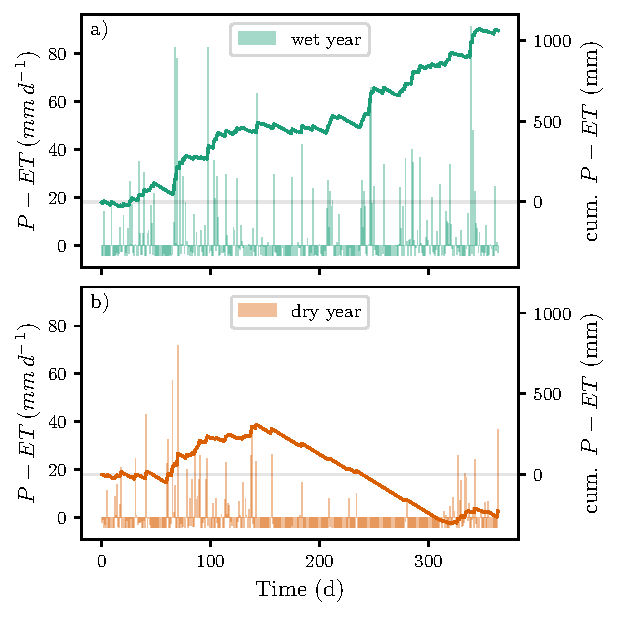
\includegraphics[width=8.3 cm]{figs/P_minus_ET.pdf}
\caption{Net water source/sink term (precipitation minus evapotranspiration) in the wet \textbf{(a)} and dry \textbf{(b)} modelled scenarios. Vertical bars show daily net water source, and the solid line shows the net cumulative sink/source of water.  Note that only the baseline evapotranspiration of $ET = 4.17$ \unit{mm d^{-1}} is shown here; the additional contribution due to the pan evaporation term was dependent on WTD and differed across modeled scenarios.}
\label{fig:p_minus_et}
\end{figure}   

The evapotranspiration was modelled as a constant daily value plus a pan evaporation term that only became active when the WTD was close to the peat surface.
The variation of evapotranspiration in tropical peatlands is considerably smaller than that of rainfall.
This applies both to inter-annual variations in total annual evapotranspiration as well as to daily and seasonal variations within a year \citep{hiranoEvapotranspirationTropicalPeat2015, watiComparisonPanEvaporation2018}.
Evapotranspiration enters our model as a quantity relative to precipitation, which justifies our choice of a constant baseline.
This value was $ET = 4.17$ \unit{mm d^{-1}}, the mean of 7 years of measurements across tropical peatlands in different disturbance states \citep{hiranoEvapotranspirationTropicalPeat2015}.
\cite{watiComparisonPanEvaporation2018} found that pan evaporation (evaporation from ponding water) in Java and Bali could be as high as $7$ \unit{mm d^{-1}}.
Based on that, we added a pan evaporation term to the constant baseline.
This pan evaporation term increased linearly from $0$ \unit{mm d^{-1}} when the WTD was at $-10$ \unit{cm}, to $3$  \unit{mm d^{-1}} when the WTD was at $+10$ \unit{cm}.
The contribution of the added pan evaporation term for higher water levels was cut off at $3$ \unit{mm d^{-1}}.


\subsubsection{Block configurations}
Two different dam setups were modelled.
One setup, which will be referred to as  'blocked configuration' or simply 'blocked', consisted of all the 168 blocks present in the study area (see Figure \ref{fig:study_area}).
The other setup, called 'not blocked', did not contain any blocks.
The typical block is made out of surrounding peat, and covers the canal width entirely up to the local peat surface.

\subsubsection{Peat hydraulic properties}
Our description of the peat hydraulic properties was based on the findings presented in \cite{cobbHowTemporalPatterns2017}, \cite{hooijerHydrologyTropicalWetland2005} and \cite{bairdHighPermeabilityExplains2017}.
The values reported for the transmissivity and its derivative, the conductivity, $K$, vary significantly both between sites and in the vertical soil profile within the same site.
In their measurements in several Panamanian peatlands, \cite{bairdHighPermeabilityExplains2017} found  that hydraulic conductivities at a depth of around $0.5$ \unit{m} in the peat profile were in the range $K = 7.5\text{--}471.9$ \unit{m d^{-1}}.
In an Brunei peatland, \cite{cobbHowTemporalPatterns2017} found $K = 1300$ \unit{m d^{-1}} at the surface and $K = 5.2$ \unit{md^{-1}} at $30$ \unit{cm} below the surface.
The specific yield, on the other hand, varies less in the cited studies.
All values are in the range $S_y=0.29\text{--}0.68$, deeper layers of the peat profile having lower values.
To capture some of this range and the rapid vertical change in the soil profile, we chose to use a single specific yield curve and  four different transmissivity curves, which were modelled using Eqs.\eqref{eq:S_zeta} and \eqref{eq:T_zeta}.
The resulting peat hydraulic properties are shown in Figure \ref{fig:parameterizatioe}, and the sets of parameters used to generate them are listed in Table \ref{tab:peat_property_params}.

\begin{table}[t]
\caption{Parameters of the peat hydraulic properties, Eqs.\eqref{eq:S_zeta} and \eqref{eq:T_zeta}. The peat hydraulic properties resulting from these parameters are shown in Figure \ref{fig:parameterizatioe}. These two sets of parameters were used in different modelled scenarios.}
\label{tab:peat_property_params} 
\begin{tabular}{lcccc}
\tophline
\textbf{Parameter scenario} & \textbf{$s_1$} & \textbf{$s_2$} &	\textbf{$t_1$} & \textbf{$t_2$}  \\
\middlehline
1 & 0.6 & 0.5 & 50 & 2.5 \\
2 & 0.6 & 0.5 & 500 & 2.5 \\
\bottomhline
\end{tabular}
\end{table}

\begin{figure*}[t]
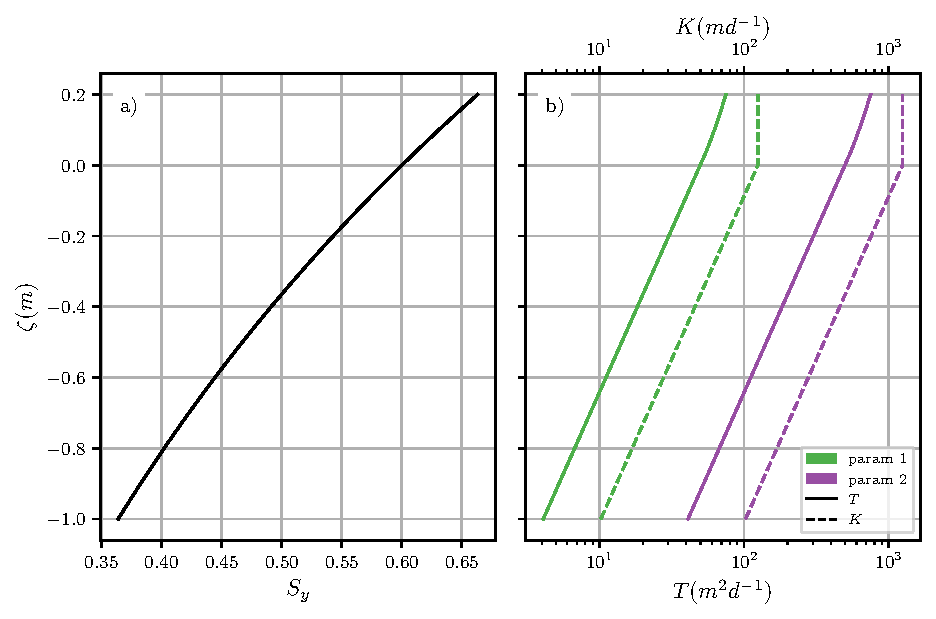
\includegraphics[width=12 cm]{figs/parameterization.pdf}
\caption{The two modelled sets of peat hydraulic properties arising from the parameters in Table \ref{tab:peat_property_params}. \textbf{(a)} Specific yield, Eq.\eqref{eq:S_zeta}, common to all modelled scenarios. \textbf{(b)} Transmissivity, Eq.\eqref{eq:T_zeta}, and conductivity, the derivative of transmissivity, $K = \frac{\partial T}{\partial \zeta}$. The different parameter sets are color coded, and this code is used in the rest of the text.}
\label{fig:parameterizatioe}
\end{figure*}

\subsubsection{Reality check}
We performed a reality check of our model by comparing the simulated WTD with the available measured field data (meteorological data from the patrol posts and dipwell data, obtained during the year 2020).
The variation in peatland topography at smaller scales than the resolution limit of our data (originally, 100 \unit{m}$\times$ 100 \unit{m}) prevented any meaningful one-to-one quantitative comparison between the modelled and the measured WTD (see Figure \ref{fig:study_area}).
This small scale variation in peat elevation is known to be of tens of centimeters \citep{lampelaGroundSurfaceMicrotopography2016, cobbHowTemporalPatterns2017}, which is comparable to daily and annual WTD ranges.

The field WTD was measured from the dipwells (see Figure \ref{fig:study_area}).
We modelled the  WTD for one year for all peat hydraulic properties using the blocked setup. 

Precipitation and evapotranspiration were determined using the data collected at the six patrol posts' weather stations (see Figure \ref{fig:study_area}).
The weather data included recordings of daily precipitation, temperature, windspeed, atmospheric pressure and relative humidity.
The daily precipitation was adopted directly from the weather station measurements.
The evaporation was modelled using the standard Penman-Montheith equation \citep{allenCropEvapotranspirationGuidelines1998}, fitting the two free parameters of the model to the annual net radiation and evapotranspiration reported in \citep{hiranoEvapotranspirationTropicalPeat2015}.
Each cell in the PHM domain received a spatially interpolated daily $P-ET$ value that was  based on its distance to the weather stations.
We chose to present here the peat hydraulic property set that best fitted the below ground range and the dynamics of measured WTD.


\subsubsection{Initial condition} \label{sec:initial-condition}
The initial WTD was the same in all modelled scenarios, including the reality check, and it was derived as follows.
Starting from total water saturation, $\zeta=0$ \unit{m} everywhere in the study area, we let the model evolve with no precipitation and a high evapotranspiration, $ET=7.5$ \unit{mm d^{-1}}.
The simulations were run with blocks and with the set of peat hydraulic properties number 4 (see Table \ref{tab:peat_property_params}).
The model was run for 50 days, recording the resulting WTD rasters at the end of each day.
We then compared the WTD  at the dipwell locations for each of the 50 rasters with the dipwell measurements from January 22nd, 2020, the first sensor measurements of the year.
The modelled WTD raster that resulted in the smallest mean squared error was selected as the initial condition for all scenarios.
Compared to other possible choices for the initial state of WTD, such as a constant WTD throughout the area, this initial condition captures the natural curvature of the WTD.


\subsection{Notation}

We will use $\langle \zeta \rangle$ to indicate the spatially averaged WTD, and $\bar{\zeta}$ to indicate the temporal average.
Additionally, the quantity 
\begin{equation} \label{eq:def_delta_zeta}
\Delta \zeta =  \zeta_{blocks} - \zeta_{no-blocks}
\end{equation}
will be used to indicate the WTD difference between two modelled scenarios that only differ by the blocking condition.

\subsection{Translation to CO\textsubscript{2} emissions}

CO\textsubscript{2} emissions in the study area were modelled as a linearly increasing function of WTD,

\begin{equation} \label{eq:m_CO2}
    m_{CO_2}(\zeta) = -a  \zeta + b,
\end{equation}
where the negative sign implies that the emissions increase with deeper WTD (note that $\zeta$ is negative below ground).
Equation \eqref{eq:m_CO2} was used for below ground WTD.
The CO\textsubscript{2} emissions resulting from above ground WTDs were set equal to the emissions at the surface, i.e., $m_{CO_2}(0) = b$. 
In this work, we used the values from \cite{jauhiainenCarbonDioxideEmissions2012}, $a=74.11$ \unit{Mg ha^{-1} m^{-1} yr^{-1}} and  $b=29.34$ \unit{Mg ha^{-1} yr^{-1}}.
These values were obtained for an Acacia plantation, which may not give the most accurate estimation of the emissions from a rehabilitating natural peat swamp forest. 
Therefore the reader is encouraged to treat the CO\textsubscript{2} emission results as a rough estimation of their magnitude.

Following the notation introduced in Eq.\eqref{eq:def_delta_zeta}, we will denote the difference in CO\textsubscript{2} emissions due to the block influence by $\Delta m_{CO_2}$.

%It follows by linearity of Eq.\eqref{eq:m_CO2} that the yearly CO2 emissions averaged over all the study area are equivalent to computing Eq.\eqref{eq:m_CO2} with the average WTD, i.e.,

%\begin{equation} \label{eq:m_CO2_linearity}
%\langle m_{CO_2}(\zeta) \rangle = m_{CO_2}(\langle \zeta \rangle).
%\end{equation}

%%%%%%%%%%%%%%%%%%%%%%%%%%%%%%%%%%%%%%%%%%
\section{Results}

\subsection{Reality check}
The comparison between the modelled and the measured WTD shows similarity in the range and  the dynamics of WTD, as shown in Figure \ref{fig:modelled_vs_measured} (a).
The deepest WTD in both measured and modelled scenarios was about $-1.5$ \unit{m}.
During most of the year WTD was between $-0.4$ \unit{m} and 0.1 \unit{m} in the majority of the measuring locations.
There were two groups of outliers in the sensor data.
The sensors with an annual WTD average below -0.7 \unit{m} all corresponded to the easternmost patrol post transect.
Three other sensors recorded an annual WTD average above 0.5 \unit{m}, but we could not find any pattern to those extreme measurements.
% The daily fluctuations produced by variations in precipitation and evapotranspiration were comparable in their magnitude.
The magnitude of the WTD rise after heavy rainfalls and the WTD drop in the recession periods were similar in magnitude in the modelled and measured datasets.
The water rise and recession slopes were similar as well.
As a result, the distribution of annually averaged modelled WTD was very similar to the measured one, as can be seen in Figure \ref{fig:modelled_vs_measured} (b).

The model captured the relevant water flow dynamics during the reality check, and thus it is considered to be plausible under the other weather scenarios presented in the study.

%\begin{figure}[t]
%\includegraphics[width=8.3 cm]{figs/reality_check_wtd_several_days.png}
%\caption{Is this fig ok?}
%\label{fig:reality_check_wtd_different_days}
%\end{figure}   


\begin{figure}[t]
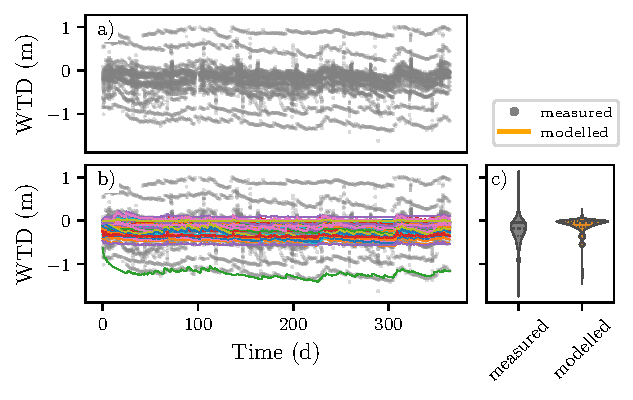
\includegraphics[width=12 cm]{figs/reality_check.pdf}
\caption{Outcome of the reality check. \textbf{a)} Measured WTD at the 141 dipwells (grey dots). \textbf{b)} Modelled WTD (coloured lines) plotted over the measured WTD of a) (grey dots) at the same locations. \textbf{c)} Kernel density estimation of measured and modelled WTD in a) and b). The dotted lines indicate the quartiles of the distribution.}
\label{fig:modelled_vs_measured}
\end{figure}   

\subsection{Block  impact on WTD}
Blocks led to a net rise of the WTD in all modelled scenarios.
This is shown qualitatively in Figure \ref{fig:diff_averaged_over_everything}, which aggregates  $\Delta \bar{\zeta}$ from all modelled scenarios into a single raster.
The existence of more areas with a positive $\Delta \bar{\zeta}$ (colored in blue in Figure \ref{fig:diff_averaged_over_everything}) means that, overall, blocks produced a net WTD rise across all the modelled scenarios.
Averaging over all modelling scenarios, the net average WTD rise was $1.51$ \unit{cm}. 
Despite the overall WTD rise, in some areas blocks had the effect of lowering WTD compared to the non-blocked scenario (colored in red in Figure \ref{fig:diff_averaged_over_everything}).
It is also remarkable that the WTD in most of the peatland area far enough from canals was practically unaffected by the presence or absence of blocks.

\begin{figure}[t]
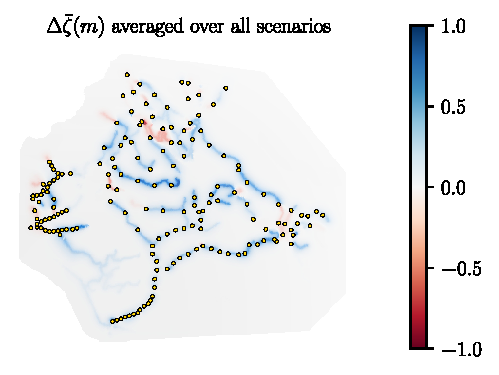
\includegraphics[width=8.3 cm]{figs/diff_averaged_over_everything_with_blocks.pdf}
\caption{Temporal average of the water table depth (WTD) difference between the blocked and non-blocked scenarios, $\Delta \bar{\zeta}$, averaged over all modelled scenarios. Blue and red colors represent the areas in which blocks raised and lowered the WTD, respectively. The grey color present in most of the study area indicates a negligible effect of the blocks on WTD far away from canals, i.e., $\Delta \bar{\zeta} \approx 0$. The block positions are represented with yellow dots.}
\label{fig:diff_averaged_over_everything}
\end{figure}   

%% in the rest of this section we untangle the role of weather and peat hydraulic properties in the dam rewetting ability.

The spatially averaged block-induced WTD rise, $\langle \Delta \zeta \rangle$, differed significantly across different hydraulic property values and weather scenarios, as shown in Figure \ref{fig:combined_wtd_and_diff_weathers_and_params}.
However, $\langle \zeta \rangle$ was always higher with the blocks than without the blocks (positive $\langle \Delta \zeta \rangle$) for all modelled scenarios.
In other words, the overall rewetting impact of the blocks was positive at all times during the simulated period, regardless of weather conditions or peat hydraulic properties. 

Block impact on WTD was greater in dry periods, when external water input to the system was scarce.
Differences between blocked and non-blocked WTD increased with prolonged dry conditions and decreased with rainfall events.
The extreme drought starting around day $150$ in the dry weather scenario provides a good example of this effect.
As the dry period progressed, the gap between blocked and non-blocked WTD kept expanding for all peat hydraulic properties (Figure \ref{fig:combined_wtd_and_diff_weathers_and_params} (b) and (d)).
Conversely, rainfall events reduced the difference between the WTD in the blocked and non-blocked scenarios (Figure \ref{fig:combined_wtd_and_diff_weathers_and_params} (b) and (c)).
As a result, the cumulative block-induced WTD rise averaged over peat hydraulic properties was $2.78$ times larger in dry conditions than in wet conditions (1.39 \unit{cm} versus 0.5 \unit{cm}).

Peat hydraulic properties also played an important role in the degree to which blocks were able to raise WTD.
Specifically, a larger hydraulic conductivity (or transmissivity) led to greater differences between the blocked and unblocked scenarios, in both weather conditions (Figure \ref{fig:combined_wtd_and_diff_weathers_and_params} (c) and (d)).
Averaged over the two weather conditions, the $\langle \Delta \bar{\zeta}\rangle$ obtained with parameter set 3, was 2.76 times greater than the one obtained with parameter set 2 (1.5 \unit{cm} versus 0.54 \unit{cm}).

\begin{figure*}[t]
\centering
\includegraphics[width=12 cm]{figs/combined_every_param_diff_vs_time_wet_and_dry.pdf}
\caption{Spatially averaged WTD (top) and WTD differences (bottom) between the blocked and non-blocked configurations for all the modelled scenarios. Spatially averaged WTD for wet \textbf{a)} and \textbf{b)} dry weather conditions. The solid lines correspond to the blocked scenario, and the dashed lines to the non-blocked. The shaded area between solid and dashed lines of the same color corresponds to the WTD difference between the two blocking scenarios, $\langle\Delta\zeta\rangle$, which is explicitly shown in \textbf{c)} and \textbf{d)} for clarity. Vertical bars in \textbf{c)} and \textbf{d)} show the daily net water input $P - ET$ [\unit{m d^{-1}}].}
\label{fig:combined_wtd_and_diff_weathers_and_params}
\end{figure*}   


%\begin{figure}[H]
%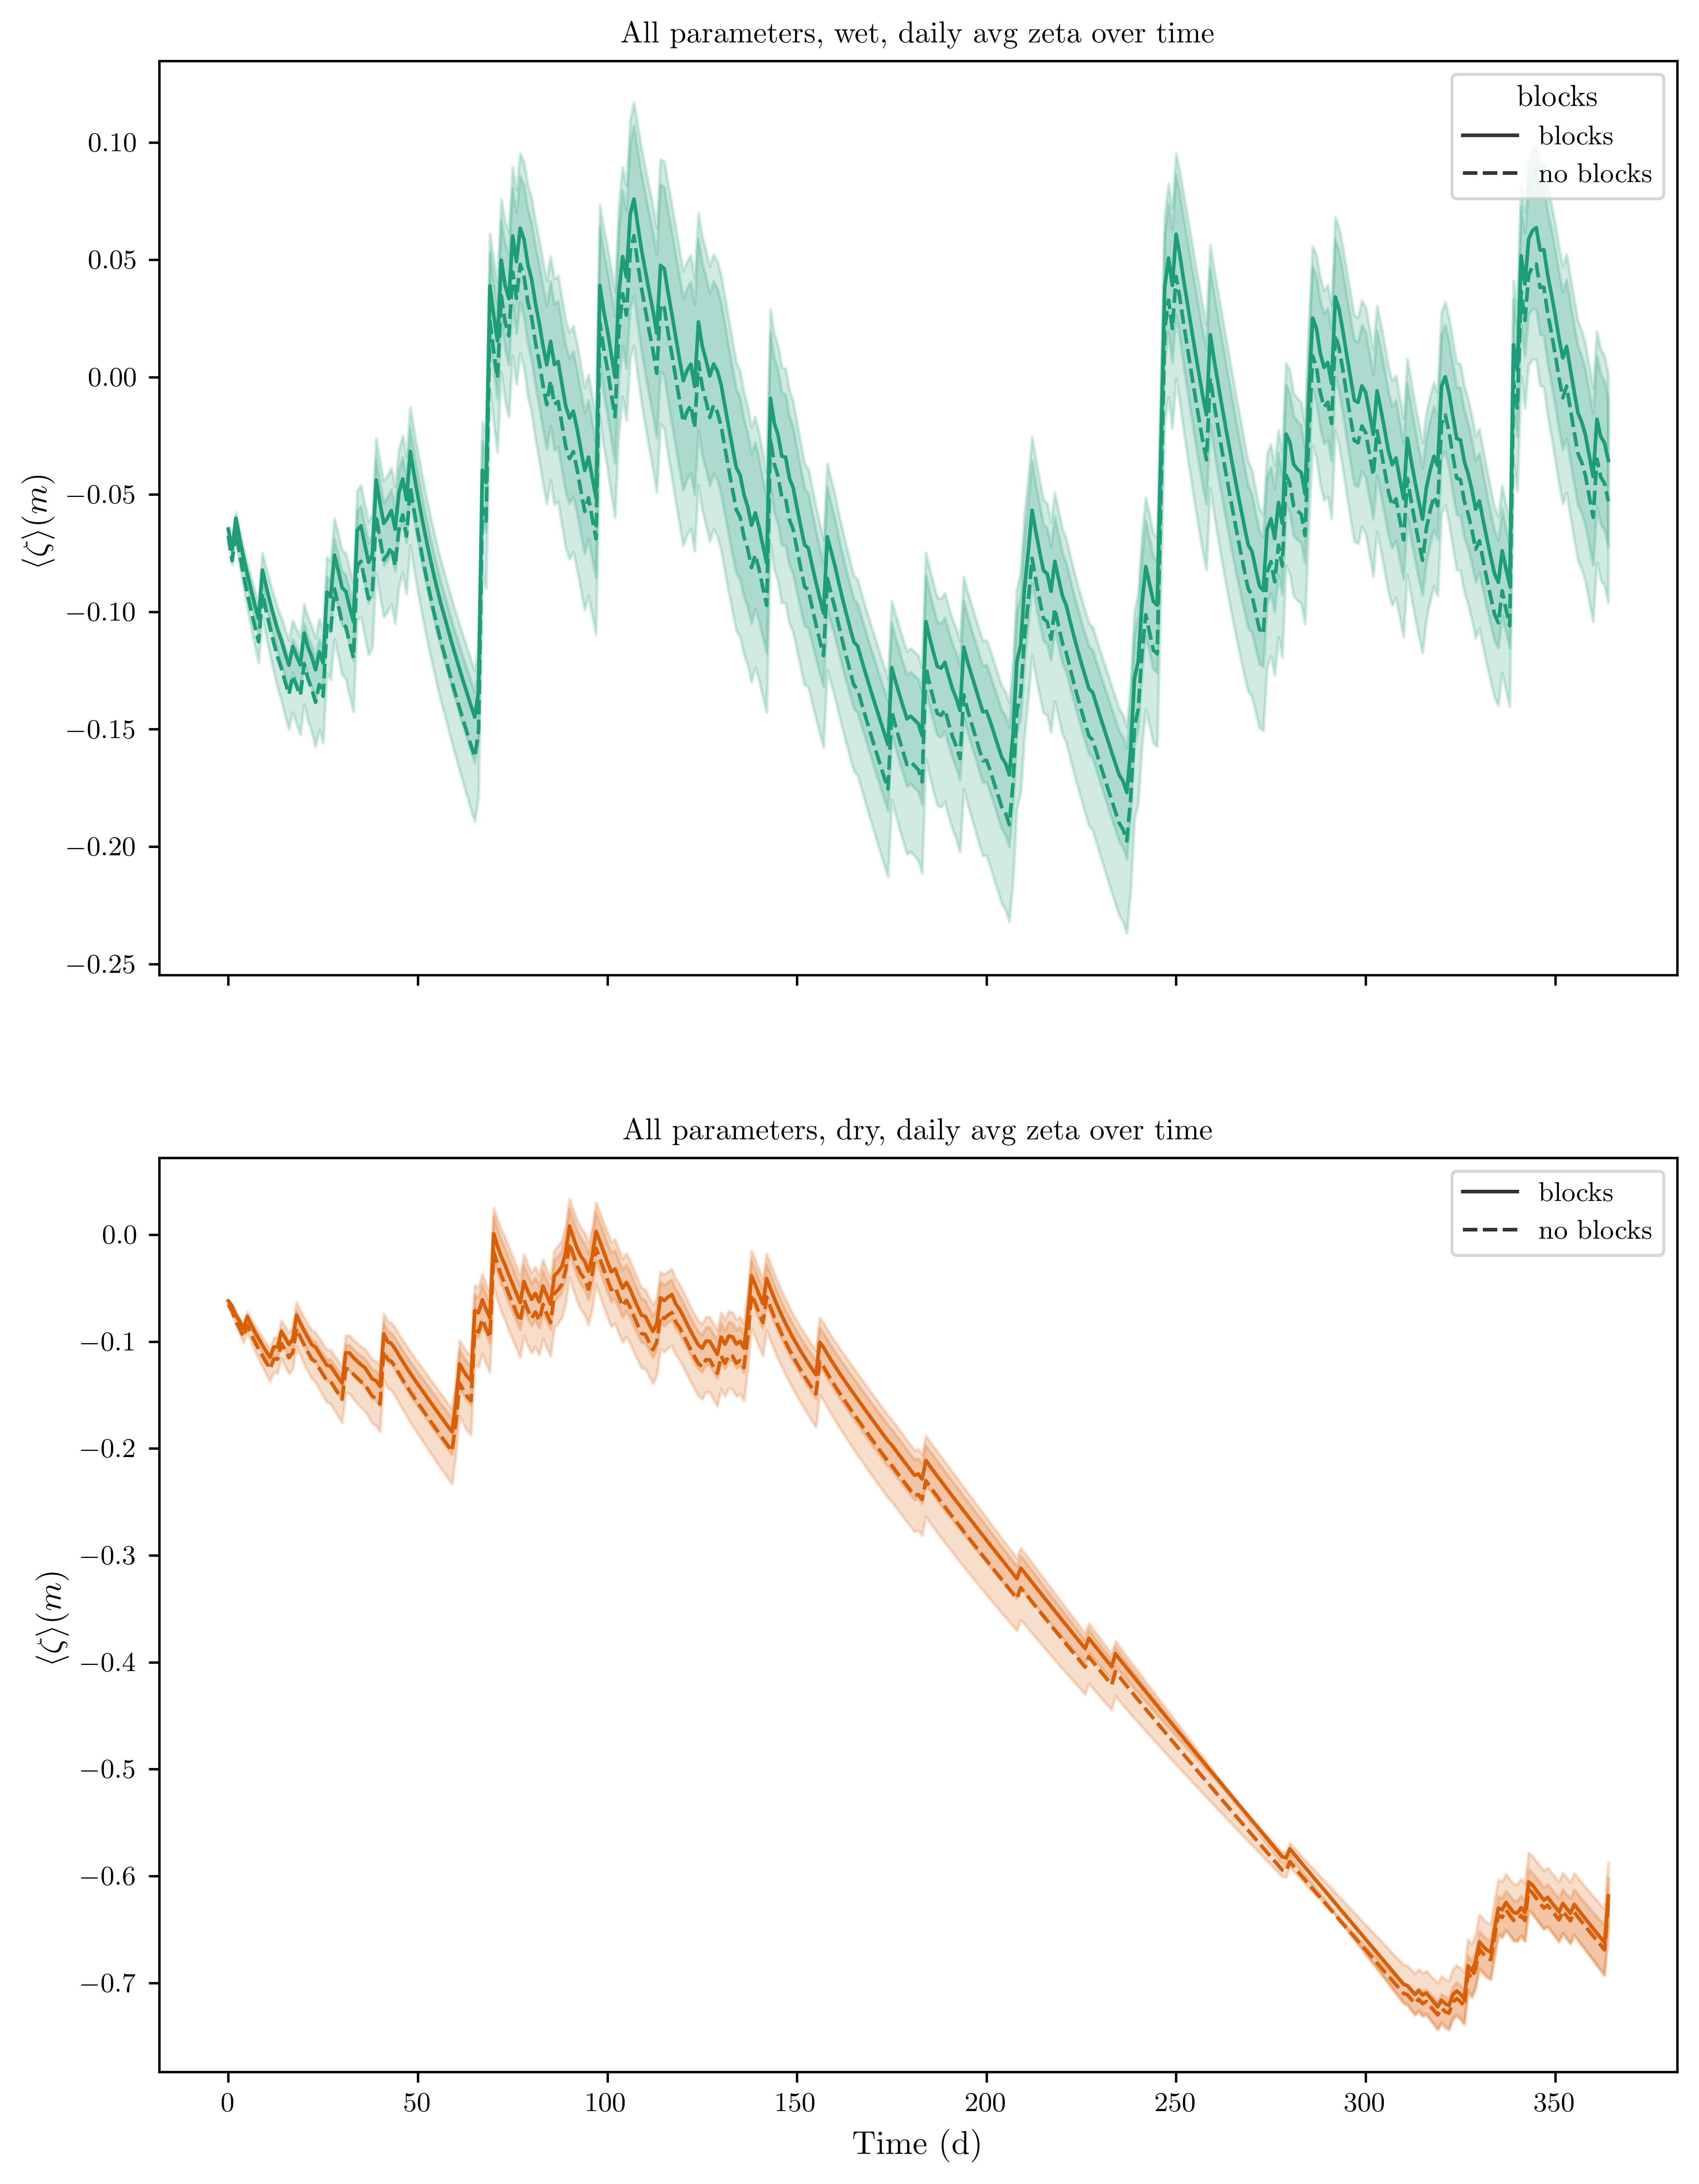
\includegraphics[width=13.5 cm]{figs/avg_zeta_vs_time_wet_and_dry_all_params.png}
%\caption{Average WTDs in wet and dry scenarios, with and without blocks. Averaged over all parameters. Shaded region show standard deviation across all parameters. Maybe it is a better idea to stay with differences between WTDs, and not to plot WTs at all?}
%\label{fig:avg_wtd_dry_and_wet}
%\end{figure}   

There was remarkable variation in the spatial extent of  block influence among the different modelling scenarios.
As an example, we show two snapshots of $\Delta \zeta$ for the same peat hydraulic properties, parameter set 3, in wet and dry years in Figure \ref{fig:spatial_extent_of_block_effect} (b) and (c).
These figures qualitatively show that the WTD difference due to the blocks at the end of the wet year was small and concentrated around canals.
In contrast, the differences at the end of the dry year were both more pronounced and extended further spatially.
Note that both the positive and the negative block impacts were larger at the end of the dry year, i.e., $\Delta \zeta$ was larger in absoulte value.
The dependence of $\Delta \bar{\zeta}$ on the distance to the nearest block, shown in Figure \ref{fig:spatial_extent_of_block_effect} a), provides a more quantitative description of the spatial extent of block impact.
The effect of blocks on WTD for all modelled scenarios was relevant until about $600$ \unit{m} from the nearest dam, and it markedly decreased from there.
The mean annual impact of the blocks on WTD more than one kilometre away was negligible (not shown in Figure \ref{fig:spatial_extent_of_block_effect} (a) for clarity).
This was true across all weather conditions and peat hydraulic properties, albeit with small variations between modelled scenarios.
Drier conditions and higher hydraulic conductivities had the effect of increasing the spatial extent of the influence of blocks.

\begin{figure}[t]
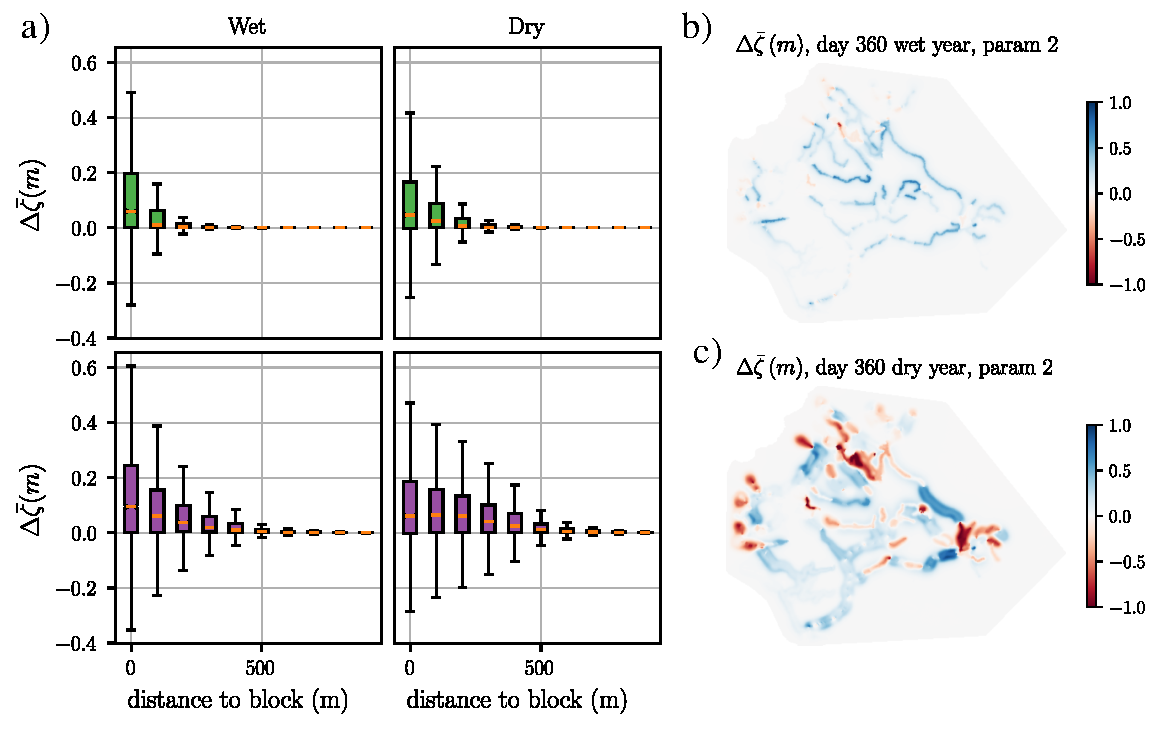
\includegraphics[width=12 cm]{figs/rasters_and_distance_to_blocks.pdf}
\caption{Spatial extent of the impact of blocks  on WTD. \textbf{a)} Temporal average of $\Delta \zeta$ plotted against the distance to the nearest block, categorized in $100$ \unit{m} classes. The box plot extends from the first to the third quartile, with an orange line at the median. The whiskers extend until 1.5 times the inter-quartile range. \textbf{b)} and \textbf{c)} show a snapshot of $\Delta \zeta$ at day $360$ of the wet \textbf{b)} and dry \textbf{c)} years for the high-transmissivity set of peat hydraulic properties (parameter number 2).}
\label{fig:spatial_extent_of_block_effect}
\end{figure}   


\subsection{Potential to decrease CO\textsubscript{2} emissions}
The net block-induced WTD rise in all modelled scenarios led to an overall decrease of CO\textsubscript{2} emissions, Figure \ref{fig:cum_CO2}.
In the worst performing rewetting scenario, with wet conditions and a peatland with the lowest studied hydraulic conductivity (parameter set 2), the non-blocked setup emitted an annual total of $0.28$ \unit{Mg ha^{-1}} more than the blocked one.
In contrast, in the best-performing scenario (dry conditions, parameter set 3) the block-induced WTD rise was translated into $1.65$ \unit{Mg ha^{-1} y^{-1}} CO\textsubscript{2} emission reduction.
Averaging over all peat hydraulic properties, the emission of $0.37$ \unit{Mg ha^{-1}} and $1.03$ \unit{Mg ha^{-1}} CO\textsubscript{2} was prevented in the whole year for dry and wet years, respectively.


\begin{figure}[t]
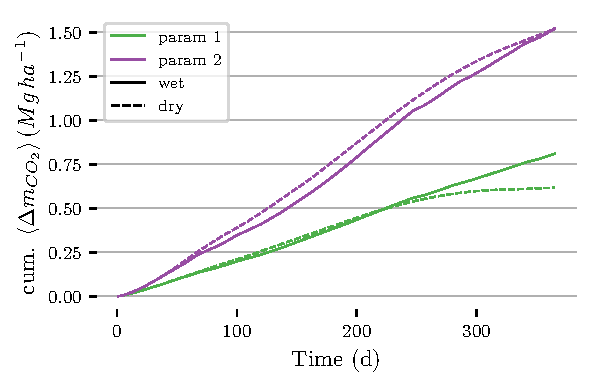
\includegraphics[width=8.3 cm]{figs/all_params_daily_cumulative_CO2.pdf}
\caption{Cumulative change in CO\textsubscript{2} emissions due to the blocks, $\Delta m_{CO_2}$ [\unit{Mg ha^{-1}}], in all modeling scenarios. Positive values indicate less CO\textsubscript{2} emissions in the blocked scenario. Solid and dashed lines correspond to wet and dry weather conditions, while colors stand for different sets of hydraulic peat properties. Sequestered CO\textsubscript{2} was computed using a linear relationship with WTD, Eq.\eqref{eq:m_CO2}.}
\label{fig:cum_CO2}
\end{figure}   


\section{Discussion}

\subsection{Comparison to previous studies}
A pursuit to estimate the impact of canal blocking in the restoration of tropical peatlands should meet the following four criteria.
First, it should capture the complex and interconnected hydrological processes influencing the block performance.
Second, the estimation should be done at spatio-temporal scales similar to the specific scale of the  restoration project.
Third, a method to meaningfully compare blocked and non-blocked scenarios is needed.
Finally, in order to make generalizable claims the sensitivity to weather conditions and peat hydraulic properties should be accounted for.

These criteria are best satisfied with a combination of empirical methods and process-based modelling.
If successful, process-based models are  able to combine the relevant  physical processes governing water flow at sufficiently large scales.
Additionally, they offer a direct method to compare different blocking setups and the ability to study the impact of different weather scenarios and peat hydraulic properties.
To our knowledge, the present work, which builds upon our previous study \citep{urzainkiCanalBlockingOptimization2020}, is the first that tries to meet all the aforementioned criteria in tropical peatlands.

A few studies have modelled tropical peatland WTD \citep{cobbHowTemporalPatterns2017, cobbScalarSimulationParameterization2019, bairdDigiBogPeatlandDevelopment2012, bairdHighPermeabilityExplains2017, morrisDigiBogPeatlandDevelopment2012, wostenTropicalPeatlandWater2006}, but to our knowledge only three have focused on the effectiveness of canal blocks: \cite{jaenickePlanningHydrologicalRestoration2010}, \cite{ishiiGroundwaterPeatland2016} and \cite{putraModellingPerformanceBunds2022}.
Both \cite{jaenickePlanningHydrologicalRestoration2010} and \cite{ishiiGroundwaterPeatland2016} modelled WTD in large areas, and reported that the  effect of dams on  WTD markedly decayed at 1 \unit{km} distance from the canals.
However, neither of the two works analyzed the effect of different  peat hydraulic properties or weather scenarios.
The only study that is comparable in scope to ours is \cite{putraModellingPerformanceBunds2022}.
Nevertheless, their study area was several orders of magnitude smaller ($20$ \unit{ha}), and their CWL was not dynamic, but manually fixed to field measurements.

The  novelty introduced by our discretization of the open channel flow equations is also worth underlining.
Unlike traditional methods in which junction nodes require a special treatment \citep{cungePracticalAspectsComputational1980, novakHydraulicModellingIntroduction2010}, our approach describes the water flow at all nodes of the computational domain with the same equation, Eq.\eqref{eq:openchannelflow-final-discretization}.
Our method is automatically applicable to canal networks of arbitrary topology, thus simplifying the model domain building process.
%To the extent that they describe mass and energy conservation laws, both methods should produce equivalent water flows at junctions.
%This feature of our model is also an improvement over other solution methods for  the open channel flow equations at junctions, such as the approach by \cite{zhu_simple_2011}.
%Compared to the model developed by \cite{zhu_simple_2011}, however, our approach is  less computationally efficient for large and complex canal networks, since the system of equations to solve has the same shape as the one arising from the traditional discretization.

\subsection{Block impact on WTD}
Five main outcomes can be drawn from the present study.

First, dams were, on average and across all the modelled scenarios, beneficial for the rewetting of the study area.
This has been observed in many studies in tropical and temperate peatlands \citep{putraEffectsDitchDams2021, sutiknoEffectivenessCanalBlocking2019, sutiknoWaterManagementHydrological2020, holdenImpactDitchBlocking2017, planas-clarkeEffectWaterTable2020, schimelpfenigEffectivenessDitchBlockage2014, kasihRewettingDegradedTropical2016}.
Canal blocks are mechanisms that increase water residence time in the peatland system and, as a result, they can only raise the average WTD.
In turn, assuming a strictly positive impact of WTD rise in CO\textsubscript{2} emission reduction, this implies that dams must reduce CO\textsubscript{2} emissions overall.
However, in line  with previous studies \citep{putraEffectsDitchDams2021, putraModellingPerformanceBunds2022}, dams were not enough to maintain WTD above the $-40$ \unit{cm} limit set by the Indonesian Peatland Regulation Agency  everywhere in the peatland during the extremely dry year (see Republic of Indonesia Government Regulation No. 57 Year 2016 about Peatland Ecosystem Protection and Management, 2016).

Second, despite raising the WTD on average, blocks did not do so everywhere in the study area.
In some areas downstream from the dams, the WTD was systematically lower in the blocked scenario than in its non-blocked counterpart.
To our knowledge, such an effect has not been reported in the literature.
Our interpretation of this result is straightforward.
The function of dams is to block water, and thus they may reduce water supply to areas with a specific combination of local canal network topology and peat topography.

Third, we found that the impact of dams on WTD was  confined to areas close to the blocks.
The WTD difference between the blocked and non-blocked scenarios was, on average, 3 \unit{cm} at 400 \unit{m} from the canals, and it was 1 \unit{mm} at a 1 \unit{km} distance (see Figure \ref{fig:spatial_extent_of_block_effect}).
Several studies support this claim \citep{sutiknoEffectivenessCanalBlocking2019, sutiknoWaterManagementHydrological2020, evansRatesSpatialVariability2019, putraEffectsDitchDams2021, putraModellingPerformanceBunds2022, ishiiGroundwaterPeatland2016, jaenickePlanningHydrologicalRestoration2010}.
\cite{sutiknoEffectivenessCanalBlocking2019}, using dipwell measurements, claimed that the radius of action of dams in tropical peatlands is around $170$ \unit{m}, and  \cite{ishiiGroundwaterPeatland2016} found the modelled WTD rise due to blocks to be about 10 \unit{cm} at a distance of 400 \unit{m}.
On the one hand, this result confirms that canal blocks are effective in raising the WTD close to the canals, which is where they are most needed.
On the other hand, it suggests that naively extrapolating WTD measurements performed in the vicinity of the canals may lead to an incorrect assessment of the ability of blocks to raise WTD throughout the study area.

Fourth, peat hydraulic conductivity had a great impact in the extent to which dams were able to raise the WTD.
This effect was also observed in \cite{putraModellingPerformanceBunds2022}, where blocks had more impact in the higher conductivity site.
Peat hydraulic properties govern the dynamics of groundwater flow and, in particular, the conductivity (or, in our model, the transmissivity) determines the rate of horizontal water flow \citep{hillelEnvironmentalSoilPhysics1998, bearModelingGroundwaterFlow2010}.
It follows that higher conductivities result in greater responses of WTD to modifications in the CWL.
This implies that peatlands with higher hydraulic conductivities have greater potential for greenhouse gas emission mitigation using canal blocking restoration.

Fifth, the impact of dams was greater in the dry year than in the wet year.
Heavier rainfall events led to smaller differences between the blocked and non-blocked scenarios.
Our interpretation is that in the absence of external water input, such as in prolonged dry periods, the ability of the dams to keep water in the system for a longer time becomes relevant.
In contrast, with enough water supply from precipitation, WTD rises regardless of whether dams exist or not.
This behaviour differed from the findings of Putra et al. in their small scale empirical and modelling studies \citep{putraEffectsDitchDams2021, putraModellingPerformanceBunds2022}.
Putra et al. reported a decrease in the effectiveness of blocks during dry periods because canals became completely dry and, therefore, blocks were not able to retain any water.
In our simulations the majority of the canal network never became completely dry, and thus we did not observe this effect.
However, our simple model of discharge through blocks, Eq.\eqref{eq:Qblock}, completely restricts water flow through blocks even when the water is below the canal bottom, i.e., when the canal is dry.
Thus, even if the canals in our simulation had dried out, our model would not have been able to reproduce the phenomenon observed by Putra et al.
The conclusion that can be drawn from the combination of the two studies is the following.
The WTD difference between the blocked and non-blocked scenarios is greater in the absence of rainfall.
Blocks are likely to delay the point in which canals become dry, yet, once that point is reached, blocks cease to have any impact on WTD.


\subsection{Model limitations}

Applications of process-based models have two main sources of uncertainty: the simplifying assumptions made in the construction of the model, and the uncertainty in the input data.

The PHM and the CNM use well-established partial differential equations to approximate water flow in peat and in canals.
Despite being two dimensional, the groundwater flow equation of the PHM has been shown to accurately represent water movement in such domains where the width exceeds the thickness \citep{connortonDoesRegionalGroundwaterflow1985}.
The two dimensional approximation has been used extensively in modelling of hydrology in tropical peatlands \citep{bairdDigiBogPeatlandDevelopment2012, cobbHowTemporalPatterns2017}.
When building the CNM we tested the diffusive wave approximation against the full open channel flow equations (Preissmann method, \cite{cungePracticalAspectsComputational1980, haahtiUnsteadyFlowSimulation2014}), and concluded that the diffusive wave approximation was accurate enough for this application (testing not shown in this study). 
This was, in part, because the daily timestep was long enough to remove the effect of the inertial terms present in the full open channel flow equations.
As was pointed out previously, the blocks were modelled as watertight barriers that extend from the surface until the impermeable bottom, while in reality they are relatively porous \citep{osakiTropicalPeatlandEcosystems2016, ritzemaCanalBlockingStrategies2014}.
The coupling between the PHM and CNM approximates water balance, but it does not strictly conserve mass.
However, this is an unavoidable drawback of any hydrological model that solves groundwater and surface water flow in different modules \citep{barthelGroundwaterSurfaceWater2016}. 

The lack of information about the water flow at the area boundaries hindered the choice of appropriate boundary conditions both in the PHM and the CNM.
In particular, there was no data on the water discharge at the catchment outlet, and we set the boundary conditions in the CWL at that point to no-flow Neumann.
This choice, although striking at first, is overrun in the PHM step by the fixed $-0.2$ \unit{m} Dirichlet boundary conditions.

The   Dirichlet boundary conditions are themselves a source of inaccuracy in the simulated WTD, as would be the case with any choice of boundary conditions.
It seems plausible to us that the  distance to which the signal of the Dirichlet boundary conditions can propagate may be similar to the distance to which a change in the CWL affects WTD.
Given our results in the present study, we can estimate that inaccuracies introduced by the Dirichlet boundary conditions would only affect the WTD up to a 1 km buffer zone around the boundaries of the study area.
We nevertheless argue that these inaccuracies do not undermine the results presented in this work because they are based on direct comparisons between different scenarios.
Indeed, the WTD difference maps displayed in Figures \ref{fig:diff_averaged_over_everything} and \ref{fig:spatial_extent_of_block_effect} (b) and (c) confirms that the difference between scenarios is negligible at the study are boundaries.
It is reasonable to think then that most of the error introduced by the boundary conditions does not have a large effect in our results.

Despite being crucial for the understanding of water dynamics, there exist few published measurements of the physical parameters which govern water flow in tropical peat and in canals.
Whereas the variability of the peat hydraulic properties was taken into account through the different modelling scenarios, the physical parameters governing open channel flow were fixed in all the scenarios. 
In reality, all these --the width, depth and cross-section shape of the canals, the block discharge coefficient, the Manning friction coefficient-- vary spatially and/or temporally.
Since the value of these coefficients have a direct influence on water dynamics, more experimental work is needed to correctly quantify the open channel flow coefficients for tropical peatlands.

All parameters of the model are expected to have some spatial variability.
Peat hydraulic properties are known to vary with vegetation and land use  \citep{bairdHighPermeabilityExplains2017, kurniantoInfluenceLandcoverChanges2019}; canal geometry changes throughout the canal network \citep{ritzemaCanalBlockingStrategies2014, osakiTropicalPeatlandEcosystems2016}; even precipitation and evapotranspiration may change over the study area \citep{vijithSpatialTemporalCharacteristics2020}.
Our model could accommodate all this spatial variability, but in the absence of data we were forced to assume constant values throughout the study area.

The model validation against the dipwell-measured WTD was limited by the coarse resolution of the PHM computational domain.
The original resolution of our digital elevation model was 100 \unit{m} $\times$ 100 \unit{m}, a scale in which tropical peat surface typically presents variations of the order of tens of centimetres \citep{lampelaGroundSurfaceMicrotopography2016}.
In the absence of further information about the precise  elevation of the dipwells, we assumed an uncertainty of comparable magnitude in the dipwell WTD measurements.
And since WTD  variation at any location was also of  tens of centimetres (see Figure \ref{fig:modelled_vs_measured}), this uncertainty prevented any direct quantitative comparison between the modelled and measured WTD.
It should also be mentioned that we are not sure about the origin of the dipwell measurements showing WTD up to 1 m above the surface in Figure \ref{fig:modelled_vs_measured}.
It could be due to a wrong datum, or to local depressions that are unnoticeable in the DTM which are canalizing the water to certain spots.
As a result, we  resorted to doing a qualitative estimation of the model plausibility.
Two main features of the reality check of Figure \ref{fig:modelled_vs_measured} support the validity of the model.
First, the model was unbiased and the range of modelled and measured WTD was comparable.
Second,  the modelled WTD presented similar ranges and slopes in the daily dynamics driven by precipitation and evapotranspiration.

%Correctly keeping track of all the system water inputs and outputs is crucial for the overall water balance, but it is a difficult task.
%There are three ways in which water can enter or exit our model: the sink/source precipitation and evapotranspiration terms in Eq.\eqref{eq:boussinesq}; the overall Dirichlet boundary conditions in the PHM; and the potential numerical inaccuracies in the interface between the CNM and the PHM.

Despite the presented limitations, we claim that the modelling setup presented here has a greater potential to study the rewetting potential of blocks than purely experimental studies have.
On the one hand, the effect of some of the aforementioned uncertainties might be partially compensated by the fact that we have only presented relative comparisons between blocked and non-blocked scenarios.
On the other hand, our model gives theoretically coherent estimates of the dam impact throughout the area, which is not possible to do  with  experimental studies alone.

\subsection{Further study}
%Several gaps in our knowledge need to be filled before we can make more general claims about the effectiveness of canal blocking restoration practices.
The present work was limited to the analysis of a single study area, with one block location configuration, for a relatively short period of time.
Future studies might consider how varying the number of dams and their positions affects WTD, since, as we know,  the dam position is critical \citep{urzainkiCanalBlockingOptimization2020}.
Furthermore, the impact of blocks on WTD would probably change in timescales of decades, which is closer to the typical lifespan of canal blocks \citep{ritzemaCanalBlockingStrategies2014, dohongReviewTechniquesEffective2018}.
When analyzing long-term scenarios, the effect of climate change in precipitation and evapotranspiration \citep{gallego-salaLatitudinalLimitsPredicted2018, wangPotentialShiftCarbon2018, caiIncreasingFrequencyExtreme2014, portnerClimateChange20222022}, as well as peat subsidence \citep{evansRatesSpatialVariability2019, hoytWidespreadSubsidenceCarbon2020, evansLongtermTrajectoryTemporal2022} will need to be addressed.
In order to have a more precise estimate of greenhouse gas emissions, future studies should take into account emissions of other compounds, such as methane and nitrous oxides.
In fact, having shallower WTD as the only optimization goal may not be desirable due to increased methane emissions---although we are not aware of any studies where methane emissions have been shown to surpass CO\textsubscript{2} emissions \citep{tehSeasonalVariabilityMethane2017, wongMicrometeorologicalMeasurementMethane2018, planas-clarkeEffectWaterTable2020, deshmukhImpactForestPlantation2020, deshmukhConservationSlowsEmission2021, kiuruPeatMacroporeNetworks2022, zouRewettingGlobalWetlands2022, lestariRewettingTropicalPeatlands2022}.

\conclusions  %% \conclusions[modified heading if necessary]
We modelled the effect that canal block restoration practices had on the WTD of a 22000 \unit{ha} drained tropical peatland.
Our results show that the blocks raised WTD on average, but their effect was limited.
Block impact on WTD at a distance of 1 \unit{km} was negligible during one year of simulations, and blocks lowered the WTD in some  areas.
The effect of dams was largest during dry periods and in peat soils with higher hydraulic conductivities.
We believe that the present modelling setup, which has been designed with stakeholders' practical management questions in mind, could be adopted by local agencies aiming at a more effective and evidence-based approach to canal block based peatland restoration.
%% The following commands are for the statements about the availability of data sets and/or software code corresponding to the manuscript.
%% It is strongly recommended to make use of these sections in case data sets and/or software code have been part of your research the article is based on.





\codedataavailability{The source code and all the data except the DTM, which is property of Deltares, are available at \citet{urzainkiTxartBlockEffectiveness2022}.
Forest Carbon Pte. Ltd. (\url{https://forestcarbon.com/}) provided the data.} %% use this section when having data sets and software code available




\videosupplement{Animations of $\Delta \bar{\zeta}$ for all modelled scenarios are available as supplementary material.} %% use this section when having video supplements available


\appendix
\section{Numerical scheme for the diffusive wave approximation} \label{ap-difwave}

The open channel flow equations \eqref{eq:diff-wave-mass} and \eqref{eq:diff-wave-momentum} must be solved in a  network of connected channel segments.
This connectivity gives rise to a  type of computational node that does not exist when the channel segments are modelled individually: the junction node, a node shared by more than one individual channel. 
The traditional discretization of the equations  involves writing the numerical approximations for each individual channel reach first, and then manually adding some mass and energy conservation conditions at the junction nodes \citep{cungePracticalAspectsComputational1980, szymkiewiczNumericalModelingOpen2010}.
However, in large and complex channel networks the traditional approach is tedious and error-prone, because all conservation equations at junctions need to   be introduced manually.
In this work we used a slightly different conceptual approach to derive the numerical discretization of the open channel flow equations that allows to set up the linear system directly from the channel network topology.

The first equation of the open channel flow equations, Eq.\eqref{eq:diff-wave-mass}, is the mass conservation equation.
In general, differential equations that describe conservation laws in one dimension take the form
\begin{equation} \label{eq:conservation_pde}
\frac{\partial u}{\partial t} =-\frac{\partial f(u(x,t))}{\partial x},
\end{equation}
where $u$ is the conserved quantity and $f(u)$ is the rate of flow or flux  of the conserved quantity.

Let us discretize space and time with regular meshes of width $\Delta x$ and time step $\Delta t$, and define the discrete mesh points $x_i=i\Delta x$ and $t_n=n\Delta t$, with $i$ and $n$ $\in \mathbb{N}$.
Conservative numerical methods are those that can be written as
\begin{equation} \label{eq:general-discretization-consesrvative-pde}
u_i^{n+1} = u_i^n + \frac{\Delta t}{\Delta x} \left[F(u^{n+1}_{i-p-1}, u^{n+1}_{i-p}, \dots, u^{n+1}_{i+q-1}) - F(u^{n+1}_{i-p}, u^{n+1}_{i-p+1}, \dots, u^{n+1}_{i+q})\right]. 
\end{equation}
for implicit schemes, and analogously for explicit schemes \citep{levequeNumericalMethodsConservation1992}.
In the simplest case, $p = 0$ and $q=1$, this becomes
\begin{equation} \label{eq:simplest-conservative-num-method}
u_i^{n+1} = u_i^n + \frac{\Delta t}{\Delta x} \left[F(u^{n+1}_{i-1}, u^{n+1}_{i}) - F(u^{n+1}_{i}, u^{n+1}_{i+1})\right].
\end{equation}

The function $F(u_i, u_{i+1})$, called the numerical flux function, plays the role of the average   flux of the conserved quantity $u$, $f(u)$, between $x_i$ and $x_{i+1}$ during the time interval $[t_n, t_{n+1}]$.

The system of equations arising from the discretization of Eq.\eqref{eq:simplest-conservative-num-method} may be interpreted as balance equations at every node.
Indeed, the form of Eq.\eqref{eq:simplest-conservative-num-method} ensures that what appears with a plus sign in the equation for $u_i$  must appear with a minus sign in the equation for $u_{i+1}$.
Therefore, the total quantity of the conserved variable $u$ in any region changes only due to flux through the boundaries.

We may impose this same condition for a general junction node with more than two neighbors.
Let us denote the index of the junction node as $J$, and let $in$ and $out$ be the set of nodes whose flux is incoming and outgoing from $J$, respectively.
Then, the discretized equation for the conservative method at a general junction node is
\begin{equation}
    \label{eq:junction-node-conservative-num-method}
    u^{n+1}_J = u^{n}_J + \frac{\Delta t}{\Delta x}\left[ \sum_{k\in in}F\left(u^{n+1}_k, u^{n+1}_J\right) - \sum_{k\in out}F\left(u^{n+1}_J, u^{n+1}_k\right) \right].
\end{equation}

Note that Eq.\eqref{eq:junction-node-conservative-num-method} reduces to Eq.\eqref{eq:simplest-conservative-num-method} for interior nodes.
Requiring conservativeness of the numerical scheme at junctions fully specifies the form of the discretized equations.   
Equation \eqref{eq:junction-node-conservative-num-method} provides the blueprint for a conservative numerical scheme  that is applicable to all nodes in the computational domain.

Our numerical method to solve the mass conservation equation, Eq.\eqref{eq:diff-wave-mass}, is obtained by setting the numerical flux function from node $i$ to node $k$ equal to $Q_{ik}$, the water discharge between those two nodes.
The discretization equation for any node in the channel network domain is then
\begin{equation} \label{eq:mass-consv-discretization}
h_i^{n+1} = h_i^{n} + \frac{\Delta t}{B\Delta x }\left[ \sum_{k\in in} Q_{ki}^{n+1} - \sum_{k \in out}Q_{ik}^{n+1}\right] + \frac{q_i^{n+1}}{B}.
\end{equation}
Note that in our model the channel width $B$ is the same for every node, i.e., $B_i = B$.

The second equation of the diffusive wave approximation, Eq.\eqref{eq:diff-wave-momentum}  becomes now useful.
It relates the magnitude of the discharge $Q$ to the square root of the gradient of the water elevation,
\begin{equation} \label{}
|Q| = C\left|\frac{\partial h}{\partial x}\right|^{1/2},
\end{equation}
where $C=\frac{A R^{2/3}}{n}$.

A straightforward discretization of the spatial derivative results in 
\begin{equation} \label{eq:discharge-discretization}
|Q_{ik}| = C_{ik}\left|\frac{h_i - h_k}{\Delta x}\right|^{1/2},
\end{equation}
where $|Q_{ik}|$ is the magnitude of the water discharge between nodes $i$ and $k$, and $C_{ik} = \frac{1}{2}\left(C_i + C_k\right)$.

Finally, we insert Eq.\eqref{eq:discharge-discretization} in Eq.\eqref{eq:mass-consv-discretization} to get our numerical scheme solving the diffusive wave approximation of the open channel flow equations,
\begin{equation} \label{eq:openchannelflow-final-discretization}
h_i^{n+1} = h_i^n - \frac{\Delta t}{B(\Delta x)^{3/2}}\sum_k\left[C_{ik}^{n+1}|h_i^{n+1} - h_k^{n+1}|^{1/2} \text{sign}(h_i^{n+1} - h_k^{n+1})\right] + \frac{q_i^{n+1}}{B}.
\end{equation}
The sign function accounts for the direction of the water flow, and the sum in $k$ goes over all neighbouring nodes of the node $i$. 
As we noted previously, this equation is valid for all nodes in the computational domain, including junction nodes.

With a judicious use of the information about the channel network topology (e.g., by using the adjacency matrix of the graph of canal nodes), this discretization enables a simple implementation of the diffusive wave approximations, since junction nodes do not need to be accounted for separately.

%%%%%%%%%%%%%%%%%%%%%
%%%%%%%%%%%%%%%%%%%%%

\noappendix       %% use this to mark the end of the appendix section. Otherwise the figures might be numbered incorrectly (e.g. 10 instead of 1).

%% Regarding figures and tables in appendices, the following two options are possible depending on your general handling of figures and tables in the manuscript environment:

%% Option 1: If you sorted all figures and tables into the sections of the text, please also sort the appendix figures and appendix tables into the respective appendix sections.
%% They will be correctly named automatically.

%% Option 2: If you put all figures after the reference list, please insert appendix tables and figures after the normal tables and figures.
%% To rename them correctly to A1, A2, etc., please add the following commands in front of them:

\appendixfigures  %% needs to be added in front of appendix figures

\appendixtables   %% needs to be added in front of appendix tables

%% Please add \clearpage between each table and/or figure. Further guidelines on figures and tables can be found below.



\authorcontribution{
IU and AL formulated the research goals and methods. IU developed the model code, performed the simulations and prepared the article. MP, HH and AL reviewed and editted the article. SP, JC, OW, PM and RY produced and validated the datasets.}

\competinginterests{
The authors declare that they have no conflict of interest}


\begin{acknowledgements}
The authors wish to acknowledge CSC -- IT Center for Science, Finland, for computational resources.
\end{acknowledgements}




%% REFERENCES

%% The reference list is compiled as follows:

%\begin{thebibliography}{}
\bibliographystyle{copernicus}
\bibliography{peatland_hydro.bib}

%\end{thebibliography}

%% Since the Copernicus LaTeX package includes the BibTeX style file copernicus.bst,
%% authors experienced with BibTeX only have to include the following two lines:
%%
%% \bibliographystyle{copernicus}
%% \bibliography{example.bib}
%%
%% URLs and DOIs can be entered in your BibTeX file as:
%%
%% URL = {http://www.xyz.org/~jones/idx_g.htm}
%% DOI = {10.5194/xyz}


%% LITERATURE CITATIONS
%%
%% command                        & example result
%% \citet{jones90}|               & Jones et al. (1990)
%% \citep{jones90}|               & (Jones et al., 1990)
%% \citep{jones90,jones93}|       & (Jones et al., 1990, 1993)
%% \citep[p.~32]{jones90}|        & (Jones et al., 1990, p.~32)
%% \citep[e.g.,][]{jones90}|      & (e.g., Jones et al., 1990)
%% \citep[e.g.,][p.~32]{jones90}| & (e.g., Jones et al., 1990, p.~32)
%% \citeauthor{jones90}|          & Jones et al.
%% \citeyear{jones90}|            & 1990



%% FIGURES

%% When figures and tables are placed at the end of the MS (article in one-column style), please add \clearpage
%% between bibliography and first table and/or figure as well as between each table and/or figure.

% The figure files should be labelled correctly with Arabic numerals (e.g. fig01.jpg, fig02.png).


%% ONE-COLUMN FIGURES

%%f
%\begin{figure}[t]
%\includegraphics[width=8.3cm]{FILE NAME}
%\caption{TEXT}
%\end{figure}
%
%%% TWO-COLUMN FIGURES
%
%%f
%\begin{figure*}[t]
%\includegraphics[width=12cm]{FILE NAME}
%\caption{TEXT}
%\end{figure*}
%
%
%%% TABLES
%%%
%%% The different columns must be seperated with a & command and should
%%% end with \\ to identify the column brake.
%
%%% ONE-COLUMN TABLE
%
%%t
%\begin{table}[t]
%\caption{TEXT}
%\begin{tabular}{column = lcr}
%\tophline
%
%\middlehline
%
%\bottomhline
%\end{tabular}
%\belowtable{} % Table Footnotes
%\end{table}
%
%%% TWO-COLUMN TABLE
%
%%t
%\begin{table*}[t]
%\caption{TEXT}
%\begin{tabular}{column = lcr}
%\tophline
%
%\middlehline
%
%\bottomhline
%\end{tabular}
%\belowtable{} % Table Footnotes
%\end{table*}
%
%%% LANDSCAPE TABLE
%
%%t
%\begin{sidewaystable*}[t]
%\caption{TEXT}
%\begin{tabular}{column = lcr}
%\tophline
%
%\middlehline
%
%\bottomhline
%\end{tabular}
%\belowtable{} % Table Footnotes
%\end{sidewaystable*}
%
%
%%% MATHEMATICAL EXPRESSIONS
%
%%% All papers typeset by Copernicus Publications follow the math typesetting regulations
%%% given by the IUPAC Green Book (IUPAC: Quantities, Units and Symbols in Physical Chemistry,
%%% 2nd Edn., Blackwell Science, available at: http://old.iupac.org/publications/books/gbook/green_book_2ed.pdf, 1993).
%%%
%%% Physical quantities/variables are typeset in italic font (t for time, T for Temperature)
%%% Indices which are not defined are typeset in italic font (x, y, z, a, b, c)
%%% Items/objects which are defined are typeset in roman font (Car A, Car B)
%%% Descriptions/specifications which are defined by itself are typeset in roman font (abs, rel, ref, tot, net, ice)
%%% Abbreviations from 2 letters are typeset in roman font (RH, LAI)
%%% Vectors are identified in bold italic font using \vec{x}
%%% Matrices are identified in bold roman font
%%% Multiplication signs are typeset using the LaTeX commands \times (for vector products, grids, and exponential notations) or \cdot
%%% The character * should not be applied as mutliplication sign
%
%
%%% EQUATIONS
%
%%% Single-row equation
%
%\begin{equation}
%
%\end{equation}
%
%%% Multiline equation
%
%\begin{align}
%& 3 + 5 = 8\\
%& 3 + 5 = 8\\
%& 3 + 5 = 8
%\end{align}
%
%
%%% MATRICES
%
%\begin{matrix}
%x & y & z\\
%x & y & z\\
%x & y & z\\
%\end{matrix}
%
%
%%% ALGORITHM
%
%\begin{algorithm}
%\caption{...}
%\label{a1}
%\begin{algorithmic}
%...
%\end{algorithmic}
%\end{algorithm}
%
%
%%% CHEMICAL FORMULAS AND REACTIONS
%
%%% For formulas embedded in the text, please use \chem{}
%
%%% The reaction environment creates labels including the letter R, i.e. (R1), (R2), etc.
%
%\begin{reaction}
%%% \rightarrow should be used for normal (one-way) chemical reactions
%%% \rightleftharpoons should be used for equilibria
%%% \leftrightarrow should be used for resonance structures
%\end{reaction}
%
%
%%% PHYSICAL UNITS
%%%
%%% Please use \unit{} and apply the exponential notation


\end{document}
